%%%%%%%%%%%%%%%%%%%%%%%%%%%%%%%%%%%%%%%%%%%%%%%%%%%%%%%%%%%%%%%%%%%%%
% PREAMBLE
%%%%%%%%%%%%%%%%%%%%%%%%%%%%%%%%%%%%%%%%%%%%%%%%%%%%%%%%%%%%%%%%%%%%%
%
% The following two commands will generate a PDF that follows all the requirements for submission
% and peer review.  Uncomment these commands to generate this output (and comment out the two lines below.)
%
% DOUBLE SPACE VERSION FOR SUBMISSION TO THE AMS
\documentclass[12pt]{article}
\usepackage{/Users/drchavas/Documents/LaTeX/AMS_LaTeX/ametsoc}
\usepackage{comment}
\usepackage{graphicx}
\linenumbers
%
% The following two commands will generate a single space, double column paper that closely
% matches an AMS journal page.  Uncomment these commands to generate this output (and comment
% out the two lines above. FOR AUTHOR USE ONLY. PAPERS SUBMITTED IN THIS FORMAT WILL BE RETURNED
% TO THE AUTHOR for submission with the correct formatting.
%
% TWO COLUMN JOURNAL PAGE LAYOUT FOR AUTHOR USE ONLY
%%%%\documentclass[10pt]{article}
%%%%\usepackage{ametsoc2col}
%
%%%%%%%%%%%%%%%%%%%%%%%%%%%%%%%%%%%%%%%%%%%%%%%%%%%%%%%%%%%%%%%%%%%%%
% ABSTRACT
%
% Enter your Abstract here
%%%%%%%%%%%%%%%%%%%%%%%%%%%%%%%%%%%%%%%%%%%%%%%%%%%%%%%%%%%%%%%%%%%%%
\newcommand{\myabstract}{Abstract}
%Tropical cyclones size. Axisymmetry. Radiative-convective equilibrium.}
%
\begin{document}
%
%%%%%%%%%%%%%%%%%%%%%%%%%%%%%%%%%%%%%%%%%%%%%%%%%%%%%%%%%%%%%%%%%%%%%
% TITLE
%
% Enter your TITLE here
%%%%%%%%%%%%%%%%%%%%%%%%%%%%%%%%%%%%%%%%%%%%%%%%%%%%%%%%%%%%%%%%%%%%%
\title{\textbf{\large{Equilibrium tropical cyclone size in an idealized state of axisymmetric radiative-convective equilibrium}}}
%
% Author names, with corresponding author information. 
% [Update and move the \thanks{...} block as appropriate.]
%
\author{\textsc{Daniel R. Chavas}
				\thanks{\textit{Corresponding author address:} 
				Daniel R. Chavas, Massachusetts Institute of Technology, 
				77 Massachusetts Ave. 54-1715, Cambridge, MA 02139. 
				\newline{E-mail: drchavas@gmail.com}}\quad\textsc{and Kerry Emanuel}\\
\textit{\footnotesize{Massachusetts Institute of Technology, Cambridge, Massachusetts}}
%\and 
%\centerline{\textsc{Extra Author}}\\% Add additional authors, different insitution
%\centerline{\textit{\footnotesize{Affiliation, City, State/Province, Country}}}
}
%
% Formatting done here...Authors should skip over this.  See above for abstract.
\ifthenelse{\boolean{dc}}
{
\twocolumn[
\begin{@twocolumnfalse}
\amstitle

% Start Abstract (Enter your Abstract above.  Do not enter any text here)
\begin{center}
\begin{minipage}{13.0cm}
\begin{abstract}
	\myabstract
	\newline
	\begin{center}
		\rule{38mm}{0.2mm}
	\end{center}
\end{abstract}
\end{minipage}
\end{center}
\end{@twocolumnfalse}
]
}
{
\amstitle
\begin{abstract}
\myabstract
\end{abstract}
\newpage
}
%%%%%%%%%%%%%%%%%%%%%%%%%%%%%%%%%%%%%%%%%%%%%%%%%%%%%%%%%%%%%%%%%%%%%
% MAIN BODY OF PAPER
%%%%%%%%%%%%%%%%%%%%%%%%%%%%%%%%%%%%%%%%%%%%%%%%%%%%%%%%%%%%%%%%%%%%%

\section{Introduction}

Our understanding of the dynamics of tropical cyclones (TCs) has improved considerably over the past three decades. The fundamental air-sea interaction instability that underlies their existence has been identified and placed within the context of a more general theory of tropical cyclones as an Carnot heat engine \citep{Emanuel_1986}. Furthermore, both theory and relatively simple dynamical models \citep{Emanuel_1995a, Rotunno_Emanuel_1987} can reproduce the characteristic features of mature tropical cyclones, including maximum wind speed, central sea level pressure, and thermodynamic structure. Most recently, \cite{Emanuel_Rotunno_2011} derived a full analytical solution for the radial structure of the balanced tropical cyclone wind field.

However, this latest solution remains defined relative to a single free parameter: the outer radius, $r_0$. Indeed, despite wide recognition of the sensitivity of both storm surge \citep{Irish_Resio_Ratcliff_2008} and wind damage \citep{Iman_Johnson_Watson_2005} to storm size, size remains largely unpredictable, and relatively little observational or modeling work has been performed to try to elucidate the factors underlying its variability. In the absence of land interaction, size is observed in nature to vary only marginally during the lifetime of a given tropical cyclone prior to recurvature into the extra-tropics \citep{Merrill_1984, Frank_1977, Chavas_Emanuel_2010, Cheng-Shang_Cheung_Wei-Ting_Elsberry_2010}, but significant variation exists from storm to storm, regardless of basin, location, and time of year.  Size is found to only weakly correlate with both latitude and intensity \citep{Merrill_1984, Weatherford_Gray_1988, Chavas_Emanuel_2010}, as the outer and inner core regions appear to evolve nearly independently.  \cite{Chavas_Emanuel_2010} found that the global distribution of $r_0$ is approximately log-normal, though distinct median sizes exist within each ocean basin, suggesting that the size of a given TC is not merely a global random variable but instead is likely modulated either by the structure of the initial disturbance, the environment in which it is embedded, or both.

Recent research has begun to explore the sensitivity of storm size to local thermodynamic variables. Observationally, \cite{Quiring_Schumacher_Labosier_Zhu_2011} combine the Extended Best Track and NCEP/NCAR Reanalysis datasets to demonstrate that various local environmental variables have at best a secondary influence on the radius of maximum wind ($r_{max}$) and the radius of gale force winds in the Atlantic basin, with the exception of a positive correlation between mid-level relative humidity and $r_{max}$.  Idealized modeling studies in \cite{Hill_Lackmann_2009} and \cite{Xu_Wang_2010} found that TCs tend to be larger when embedded in moister mid-tropospheric environments due to the increase in spiral band activity and subsequent generation of diabatic potential vorticity which acts to expand the wind field laterally. Using a simple three-layer axisymmetric model, \cite{Smith_Schmidt_Montgomery_2011} showed an optimum in storm size as a function of ambient planetary rotation attributed to the inhibitive effect of inertial stability on boundary-layer inflow as the rotation rate is increased.  Finally, the seminal work of \cite{Rotunno_Emanuel_1987} found in an idealized axisymmetric framework a strong relationship between the horizontal length scales of the initial and mature vortex.

A dynamical systems approach may provide a path forward in improving our understanding of tropical cyclone size. \cite{Tang_Emanuel_2010} demonstrated analytically that tropical cyclone intensity may be viewed as a non-linear dynamical system that evolves towards a stable equilibrium whose value depends on the local environmental and initial conditions. This behavior has been verified in a modeling context on both short time-scales (REFERENCES) and, importantly, over long time-scales over which the storm's maximum wind speed has achieved statistical equilibrium \citep{Hakim_2011}.  However, no such theory exists for the dynamical evolution of tropical cyclone structure, and the tropical cyclone at statistical structural equilibrium remains unexplored. This is of particular relevance given the large range of variation in size observed in nature \citep{Chavas_Emanuel_2010}.

Thus, this work seeks to build upon the small base of literature on tropical cyclone size by systematically exploring the sensitivity of the structure of a tropical cyclone at statistical equilibrium to the set of relevant model, initial, and environmental dimensional variables. Expanding on the work of \cite{Hakim_2011}, we perform our analysis in the simplest possible model and physical environment: a highly-idealized state of radiative-convective equilibrium (RCE). Based on the results of the sensitivity analysis, we then apply dimensional analysis to quantify how, at equilibrium, each structural variable of interest scales with the set of relevant input parameters. Section 2 details the methodology, including model description and experimental design. Results and comparison with existing theory are presented in section 3, with the potential implications of key findings discussed in section 4. Finally, section 5 provides a brief summary and conclusions.

\section{Methodology}

\subsection{Model description}
This work employs Version 15 of the Bryan Cloud Model (CM1), a non-hydrostatic atmospheric cloud-system resolving model (CSRM; original version described in \cite{Bryan_Fritsch_2002}) that has been applied to the study of a variety of convective systems including topographic flow \citep{Miglietta_Rotunno_2010}, tropical cyclones \citep{Bryan_Rotunno_2009b}, and mid-latitude squall lines \citep{Parker_2008}.  CM1 was originally written with the goal of incorporating state of the art numerics and physics, in particular for moist processes, while satisfying near-exact conservation of both mass and energy in a reversible saturated environment. The model is set up in three-dimensions but can also be configured for two-dimensional axisymmetric (radius-height) geometry, the latter of which is used here for the sake of simplicity and computational efficiency.

CM1 solves the fully compressible set of equations of motion in height coordinates on an f-plane for flow velocities ($u$, $v$, $w$), non-dimensional pressure ($\pi$), potential temperature ($\theta$), and the mixing ratios of water in vapor, liquid, and solid states ($q_\chi$) on a fully staggered Arakawa C-type grid in height coordinates. The model has a rigid lid at the top with a 5-km thick damping layer beneath; similarly, there is a wall at the domain's outer horizontal edge with an adjacent damping layer whose thickness is set to approximately $\frac{1}{15}$ of the domain's width.  Model horizontal (x-y) and vertical grid spacing are each constant in the domain. Model microphysics is represented using the Goddard-LFO scheme based on \cite{Lin_Farley_Orville_1983}, which is a mixed-phase bulk ice scheme with prognostic equations for water vapor, cloud water, rainwater, pristine ice crystals, snow, and large ice. For full details, see \cite{Bryan_Fritsch_2002}. Lastly, though the model now includes a comprehensive radiation scheme, it is replaced with an idealized scheme discussed below due to its simplicity.

For axisymmetric geometry, turbulence is parameterized using a Smagorinsky-type closure scheme \citep{Smagorinsky_1963}, which assumes steady and homogeneous unresolved turbulence, modified such that different eddy viscosities are used for the horizontal and vertical directions to represent the differing nature of turbulence between the radial and vertical directions in a highly anisotropic system such as in the inner core of a tropical cyclone.  In the context of tropical cyclones, turbulence fulfills the critical role of counteracting eyewall frontogenesis by the secondary circulation that, in the inviscid limit, would lead to frontal collapse \citep{Emanuel_1997}.


\subsection{Idealized model/environmental RCE set-up}
We construct a highly-idealized model and environmental configuration in order to reduce the model atmospheric system to its simplest possible state with the minimal number of dimensional variables. Model horizontal and vertical resolution are each set constant and no grid stretching is applied. Radiative cooling is set to a constant rate (typical of the clear-sky mean tropical troposphere, see \cite{Hartmann_Holton_Fu_2001}) everywhere in the domain above a threshold temperature, with Newtonian relaxation back to this threshold for sub-threshold temperatures:
%%FIX LINE NUMBERING PROBLEM HERE!
\begin{equation}
\label{eq:radscheme}
\frac{\partial \theta}{\partial t} = \left\{ 
\begin{array}{l l}
  - Q_{cool} & \quad \mbox{$T > T_{tpp}$}\\
  \frac{\theta(T_{tpp})-\theta}{\tau} & \quad \mbox{$T \le T_{tpp}$}\\
  \end{array} \right.
\end{equation}
where $T$ is the temperature, $T_{tpp}$ is the constant threshold temperature below which Newtonian relaxation applies, $\tau$ is the relaxation timescale, and $Q_{cool}$ is the constant radiative cooling rate and is applied to the potential temperature. Thus, all water-radiation feedbacks are neglected. The lower-boundary sea surface temperature, $T_{sst}$, is set constant. Surface fluxes of enthalpy and momentum are calculated using standard bulk aerodynamic formulae
\begin{align}
	\label{eq:enthalpyflux}
	F_k &= C_k \rho |{\bf u}|(k^*_s-k) \\
	\label{eq:sfcstress}
	\tau_s &= -C_d \rho |{\bf u}|{\bf u}
\end{align}
where $F_k$ is the surface enthalpy flux, {\bf u} is the near-surface (i.e. lowest model level) wind velocity, $k$ is the near-surface enthalpy, $k^*_s$ is the saturation enthalpy of the sea surface, $\tau_s$ is the surface stress, and the exchange coefficients for momentum, $C_d$, and enthalpy, $C_k$, are set constant, despite their acknowledged real-world dependence on wind-speed \citep{Powell_Vickery_Reinhold_2003}. Finally, although axisymmetric geometry precludes the imposition of background flow, in the case of a uniform background wind, galilean invariance dictates that its only manifestation in the dynamics of the system is through the surface enthalpy fluxes given in \eqref{eq:enthalpyflux}.  Thus, we represent this effect by simply adding a constant background wind speed, $u_s$, to {\bf u} for the model calculation of this quantity.  Note that there is an additional three-dimensional asymmetry in the surface flux calculation due to the signed summation of the background and perturbation components of the wind.  In the context of a mature tropical cyclone, for which $u_{TC} \gg u_s$, this effect is likely small and nonetheless is necessarily neglected due to the model geometry employed in this work.  This set-up is conceptually similar to that of \cite{Hakim_2011} with the important exceptions that here we employ a non-interactive radiative scheme and we include background surface fluxes throughout the domain.

This configuration provides a simplified framework for the exploration of equilibrium tropical cyclone structure in RCE. \cite{Nolan_Rappin_Emanuel_2007} found that, in the presence of a "realistic" radiation scheme, the f-plane RCE state depends only on $T_{sst}$, $u_s$ and very weakly on $f$. For this work, the idealized radiation scheme introduces two additional degrees of freedom, $T_{tpp}$ and $Q_{cool}$, to which the RCE state is sensitive. Thus, we initialize each axisymmetric simulation with the vertical profiles of temperature and water vapor calculated as the 70-100 day time- and horizontal-mean profiles from the corresponding three-dimensional simulation on a 196x196x40 km domain with identical $T_{sst}$, $T_{tpp}$, $Q_{cool}$, and $u_s$; the RCE state is indeed found to be nearly insensitive to $f$ and thus it is held constant at its control value to reduce computational load. This domain size is specifically chosen to be large enough to permit a large number of updrafts but small enough to inhibit convective self-aggregation \citep{Bretherton_Blossey_Khairoutdinov_2005} over a period of at least 100 days, though absent any water-radiative feedbacks convective aggregation is unlikely anyways. The horizontal and vertical resolutions are $dx = dy = 4 \; km$ and $dz = .625 \; km$, respectively, with doubly-periodic horizontal boundary conditions.  The stratospheric radiative relaxation time-scale is set to $\tau = 40 \; days$. This approach ensures that each axisymmetric simulation begins very close to its "natural" model-equilibrated background state (first emphasized in \cite{Rotunno_Emanuel_1987}) and thus is absent any significant stores of available potential energy that may exist by imposing an alternate initial state, such as a mean tropical sounding.

The result of the above methodology is a model RCE atmosphere comprised of a troposphere capped by a nearly isothermal stratosphere. This carries the important benefit that the tropopause height is set by a single, externally-defined temperature, $T_{tpp}$, which conveniently corresponds approximately to the convective outflow temperature central to the maximum potential intensity theory of tropical cyclones.  
The generalized potential intensity \citep{Emanuel_2010} is given by
\begin{equation}
\label{eq:vpot1}
V^2_p = \frac{C_k}{C_d}\frac{T_{sst} - T_{tpp}}{T_{tpp}}(k^*_0-k)
\end{equation}
Combining \eqref{eq:vpot1} with the surface enthalpy flux equation in \eqref{eq:enthalpyflux} gives
\begin{equation}
\label{eq:vpot2}
V^2_p = \frac{T_{sst} - T_{tpp}}{T_{tpp}}\frac{F_k}{\rho C_d |{\bf u}|}
\end{equation}
In RCE, column energy balance requires that the surface enthalpy flux into the column be exactly balanced by the column-integrated radiative cooling, which in this idealized set-up is given by
\begin{equation}
\label{eq:colenergybal}
F_k = \int^0_{p_s}{C_p\frac{\partial T}{\partial t}}dp = \int^0_{p_s}{C_p\frac{\partial \theta}{\partial t}\left(\frac{p}{p_0}\right)^{R_d/C_p}}dp\approx C_p Q_{cool} \frac{\overline{\Delta p}}{g}
\end{equation}
where $C_p$ is the specific heat of air, $\overline{\Delta p}$ is a measure of the pressure thickness of the troposphere, and we have ignored any small contribution from Newtonian relaxation in the stratosphere.  Plugging \eqref{eq:colenergybal} into \eqref{eq:vpot2} results in
\begin{equation}
\label{eq:vpot3}
V^2_p = \frac{T_{sst} - T_{tpp}}{T_{tpp}}\frac{C_p Q_{cool} \overline{ \Delta p}}{g \rho C_d |{\bf u}|}
\end{equation}
Thus, \eqref{eq:vpot3} makes it readily apparent that potential intensity in RCE with constant tropospheric cooling is a function of four externally-defined parameters: $T_{sst}$, $T_{tpp}$, $u_s$, and $Q_{cool}$, with the tropospheric thickness $\Delta p$ primarily a function of $T_{tpp}$. This fact will be leveraged in the set of experiments detailed below.


\subsection{Control run parameters}
For the control run, model parameters are $dr = 4 \; km$, $dz = .625 \; km$, $H_{domain} = 25 \; km$, $C_d = C_k = .0015$, radial mixing length $l_h = 1.5 \; km$ \citep{Bryan_Rotunno_2009b}, and vertical mixing length $l_h = .1 \; km$. Control environmental parameters are $T_{sst} = 300 \; K$; $T_{tpp} = 200 \; K$; $f = 5*10^{-5} \; s^{-1}$; $Q_{cool} = 1 \; \frac{K}{day}$; $u_s = 3 \; ms^{-1}$. All simulations are run for 100 days. The initial control run RCE sounding is displayed in Figure *SOUNDING*. The potential intensity, calculated from the initial RCE sounding using the Emanuel sub-routine with zero boundary layer wind speed reduction and including dissipative heating is $V_p = 93 \; ms^{-1}$.  This compares very well with the prediction made by \eqref{vpot3} of $92 \; ms^{-1}$ for $\rho =  1.1 \; kgm^{-3}$ and a tropospheric pressure depth of $850 \; hPa$.

Following the work of \cite{Bister_Emanuel_1997}, which demonstrated that the fundamental process during tropical cyclogenesis is the near-saturation of the column at the mesoscale in the core of the nascent storm, the simulation is initialized with a mid-level moisture anomaly above the boundary layer at constant virtual temperature in a region bounded by $z = [1.5, 9.375] \; km$ and $r = (0, r_{0_q})$ within a quiescent environment. The control value is $r_{0_q} = 200 \; km$.  We also test initialization with a mid-level vortex, of the form used in \cite{Rotunno_Emanuel_1987}, with $V_{m_0} = 12.5 \; ms^{-1}$, $r_{m_0} = \frac{1}{5} r_{0_u}$, centered at $z=4.375 \; km$ with azimuthal wind speeds above and below decaying linearly to zero over a distance of $2.875 \; km$, and a control size of $r_{0_u} = 400 \; km$. However, as is shown below, the two approaches have similar results, and thus for the sake of simplicity we elect to initialize all other simulations with the mid-level moisture anomaly.

The domain size for the control run requires special attention. Prior research modeling tropical cyclones typically place the outer wall of the domain at a distance of 1000-1500 km (e.g. \cite{Rotunno_Emanuel_1987, Hakim_2011}).  However, as shown in Figure \ref{fig:domainsize}, which depicts the quasi-steady radial profile of the azimuthal component of the gradient wind at $z = 1 \; km$, storm structure at statistical equilibrium is dramatically influenced by the radius of the outer wall up to an upper bound. Beyond this upper bound, however, the equilibrium storm is largely insensitive to the location of the wall. The theoretical basis underlying the existence of this upper bound is discussed below.

Thus, because the outer wall is purely a model artifact, we set the outer wall conservatively at $L_{domain} = 12288 \; km$ for all simulations run herein.  This has the added benefit of ensuring that the storm itself is not significantly altering the background environment, which may act to modify the potential intensity from its RCE value.

\subsection{Characterizing equilibrium storm structure}
Following the theory presented in \cite{Emanuel_Rotunno_2011}, we characterize the complete structure of the tropical cyclone wind field with three variables: the maximum gradient wind speed, $V_m$, the radius of maximum gradient wind, $r_m$, and the outer radius, $r_0$, where the wind vanishes. Importantly, only one of the size variables $r_m$ and $r_0$ is a free variable while the other is given by the analytical solution.  We first calculate a 2-day running mean of the radial profile of the azimuthal gradient wind at approximately $z = 1 \; km$ (i.e. near the top of the boundary layer), from which we create a time-series of each variable. This time averaging is necessary to reduce noise in the calculation of the gradient wind from the full pressure field, the pitfalls of which are discussed in \cite{Bryan_Rotunno_2009}. The equilibrium values are then defined as the respective 70-100 day means.  This approach allows one to check that each variable has independently reached statistical equilibrium.

%which we define here as having a 30-day running mean value within 10\% of the day 70-100 mean.

Unfortunately, even in a modeling environment, direct calculation of $r_0$ is difficult due to the noisy nature of the very outer edge of the model storm. Thus, here we follow the methodology of \cite{Chavas_Emanuel_2010} and employ the outer wind structure model derived in Emanuel (2004) to extrapolate radially outwards to $r_0$ from the radius of $12 \; ms^{-1}$. The model assumes that the flow is steady, axisymmetric, and absent deep convection beyond $r_{12}$, resulting in a local balance between subsidence warming and radiative cooling. Furthermore, given that both the lapse rate and the rate of clear-sky radiative cooling are nearly constant in the tropics, the equilibrium subsidence velocity, $w_{cool}$, can be taken to be approximately constant. In equilibrium, this subsidence rate must match the rate of Ekman suction-induced entrainment of free tropospheric air into the boundary layer in order to prevent the creation of large vertical temperature gradients across the top of the boundary layer. The radial profile of azimuthal velocity is therefore determined as that which provides the required Ekman suction, and is given by
\begin{equation}
    \label{eq:Lilly}
    \frac{\partial (rV)}{\partial r}=\frac{2r^2C_dV^2}{w_{cool}(r_0^2-r^2)}-fr
\end{equation}
where $r$ is the radius and $V$ is the azimuthal wind speed. The value of $w_{cool}$ is calculated from the assumed balance between subsidence and radiative cooling
\begin{equation}
    \label{eq:radsub}
    w_{cool} \frac{\partial \theta}{\partial z}=Q_{cool}
\end{equation}
where $\frac{\partial \theta}{\partial z}$ is set to its mean value in the layer $z=1.5-5 \; km$ (i.e. directly above the boundary layer) in the RCE initial sounding. For the control run, this gives $w_{cool} = .27 \; cm s^{-1}$, which agrees well with the value of $.23$ obtained by calculating the mean (negative) vertical velocity in the region $r = [400, 800] \; km$ and $z = [1.5, 5] \; km$ from the equilibrium state of the control simulation.  Finally, we solve for $r_0$ in \eqref{eq:Lilly} using a shooting method.

\subsection{Experimental approach: parametric sensitivities and dimensional analysis}
We begin with a simulation with a control set of dimensional parameters out to 100 days, a time period sufficient for the full storm structure to reach statistical equilibrium; the evolution of this control run is discussed below.  We then perform a wide range of experiments in which we independently and systematically vary all dimensional parameters deemed relevant to the dynamics of the system: $l_h$, $f$, $r_{0_q}$, $r_{0_u}$, $T_{sst}$, $T_{tpp}$, $Q_{cool}$, and $u_s$; the latter four are subsumed within $V_p$ as discussed in Section 3(b).  For each of $l_h$, $f$, $r_{0_q}$, and $r_{0_u}$, we run six simulations relative to the control case: three with the parameter successively halved and three successively doubled from the control value.  For $V_p$, we perform a suite of simulations with a variety of combinations of its constitutive sub-variables that, in combination, span a reasonable range of values of $V_p$.

The final scaling results then indicate to which dimensional variables the equilibrium storm structure is sensitive.  Dimensional analysis can then be applied to quantify the scaling relationship that exists between the structural variable of interest and all relevant dimensional variables simultaneously.

\section{Results}

%basic evolution; time-scale to equilibrium for each variable; equilibrium structure
\subsection{Control run}
Figure \ref{fig:timeseries} displays the time evolution of the 1-day running mean of $V_m$, $r_m$, and $r_0$ for the control simulation as well as estimated time-scales to equilibrium for each individual variable.  As noted above, equilibrium is defined simply as the 70-100 day mean value, and the time-scale to equilibrium, $\tau^*_x$, where $x$ is the variable of interest, is defined as the starting time of the first 30-day interval, iterating backwards from day 70, whose mean value is within 10\% of the equilibrium value.  All three variables exhibit similar qualitative evolutions: rapid increase during genesis to a super-equilibrium value followed by a more gradual decay to equilibrium.  However, the degree of excess over equilibrium is largest for $r_0$ ($\sim 70\%$), moderate for $r_m$ ($\sim 50\%$) and relatively small ($\sim 20\%$) for $V_m$. In the case of $V_m$, the fractional overshoot is slightly smaller than the value found in \cite{Hakim_2011} of approximately 30\% for the same radial turbulent mixing length, though \cite{Hakim_2011} analyzed the surface wind rather than the gradient wind near the top of the boundary layer.  Moreover, the time-scales to equilibrium for storm size are significantly longer for size ($\tau^*_{rm} = 54 \; days$ and $\tau^*_{r0} = 58 \; days$) than for intensity ($\tau^*_V = 30 \; days$).  The details of the transient phase of the structural evolution will be explored in a separate work.  Ultimately, the control simulation's equilibrium storm structure is characterized by $V^*_m = 73 \; ms^{-1}, r^*_m = 53 \; km, r^*_0 = 1150 \; km$.

These results suggest that modeling tropical cyclones over a period sufficient to achieve quasi-equilibrium in intensity (typically 10-20 days), as is commonly done in the literature, may result in a storm that has not reached structural equilibrium or else has done so artificially due to the domain-limitation imposed by the model's outer wall.

%parametric collapse to MPI
\subsection{Sensitivity to potential intensity}
Prior to exploring the sensitivity of storm structure to the full suite of dimensional parameters, we may first seek to exploit our relation for potential intensity in RCE given by Eq. \eqref{eq:vpot3} in order to simplify the dimensional space amenable to testing. Given \eqref{eq:vpot3}, one may hypothesize that the primary role of the dimensional parameters $T_{sst}$, $T_{tpp}$, $Q_{cool}$, and $u_s$ is to modulate the potential intensity. To test this hypothesis, we explore the sensitivity of storm structure to the potential intensity, the range of values of which is determined by independently varying each of the above four parameters over the following ranges (listed in order of increasing potential intensity; middle value corresponds to the original control case): $T_{sst} = 295, 297.5, 300, 302.5, 305 \; K$; $T_{tpp} = 250, 225, 200, 175, 150 \; K$; $u_s = 5, 4, 3, 2, 1 \; ms^{-1}$; $Q_{cool} = .25, .5, 1, 2, 4 \; K day^{-1}$.  For simulations with $T_{tpp}$ colder than the control run value, the model domain height is increased to $30 \; km$ to ensure that there is no interference between the convective outflow and the damping layer near the model top.

The resulting scaling of the maximum gradient wind speed at the top of the boundary layer with the potential intensity is shown in Figure \ref{fig:mpicollapse_V}.  In this case, in the absence of environmental conditions that might inhibit intensification (e.g. vertical wind shear, upper ocean mixing), one expects that $V_m$ ought to scale linear with $V_p$ and therefore that the scaling with the four input sub-variables should collapse to this single linear scaling, and this is indeed the case.  The fit is particularly tight for potential intensities at or below the control value.

Of greater interest, however, is the question of whether such a collapse is observed in the scaling of the size variables with $V_p$. Figure \ref{fig:mpicollapse_r} displays the scalings for $r_m$ and $r_0$, which indeed also approximately collapse to a single scaling with $V_p$, particularly for $r_0$. The largest spread exists in $r_m$ at large values of potential intensity, though the overall quasi-linear trend remains evident. Moreover, the scalings for $Q_{cool}$ are monotonic in both $V_m$ and $r_m$ but exhibit some non-linearity, with negative curvature in the former and positive curvature in the latter, suggesting a shift in $r_m$ while conserving angular momentum. Meanwhile, the scaling for $r_0$ diverges for low values of $Q_{cool}$ due to the direct dependence of the calculated radiative subsidence rate, $w_{cool}$, used to calculate $r_0$ in \eqref{eq:Lilly} on the radiative cooling rate; smaller values for $w_{cool}$ correspond to larger values for $r_0$, all else equal. To the extent that this sensitivity is exhibited primarily in the outer region of the storm (i.e. beyond $r_{12}$), this divergence indicates an important limitation on the simple three-variable representation of storm structure employed here, which does not distinguish between variability for $r_m < r < r_{12}$ and $r > r_{12}$.  Finally, there is one obvious outlier: the $T_{sst} = 305 \; K$ simulation exhibits an equilibrium storm that is larger and more intense than would be expected from the set of simulations with variable $T_{sst}$ and their associated values for $V_p$. The reason for this outlier is unclear, but the non-linear jump with increasing $T_{sst}$ may indicate a deficiency due to the coarse vertical resolution within the boundary layer.

Overall, though, the above results in combination indicate that the primary contribution of these four environmental variables to the equilibrium dynamics not only of the maximum gradient wind speed but of the entire storm structure is manifest in the potential intensity.

%sensitivity testing to all relevant parameters
\subsection{Parametric sensitivity experiments}
We may now proceed to the full parametric sensitivity experiments, where we test $V_p$ in lieu of $T_{sst}$, $T_{tpp}$, $u_s$, and $Q_{cool}$ based on the results of the previous section. Figure \ref{fig:dimscaling} displays the scaling of each structural variable with the set of relevant input parameters.  All three variables exhibit systematic sensitivity (indicated by a non-zero slope) to three parameters: the potential intensity, $V_p$, the Coriolis parameter, $f$, and the turbulent radial mixing length, $l_h$. Meanwhile, the equilibrium structure is insensitive to the initial disturbance structure as indicated by the near-zero slope in the scaling with the length scale of the initial perturbation, regardless of whether this perturbation is in the form of a mid-level positive vorticity anomaly or positive moisture anomaly.  Moreover, equilibrium storm structure is insensitive to the vertical mixing length over the range of values tested here, though for sufficiently large (and likely unphysical) values on the order of the depth of the troposphere, storm structure does indeed become sensitive to this parameter (not shown) as strong vertical mixing across sloped angular momentum contours within the eyewall has a strong impact on the structure of a mature storm.

Closer inspection of the systematic sensitivities reveals some interesting details about the individual scalings. First, as would be expected, $V_m$ is most strongly modulated by the potential intensity, with a simple linear relationship of unit slope. $V_m$ is weakly negatively correlated with the radial mixing length, with maximum wind speed doubling only once over the entire scaling range. This latter sensitivity reflects the simple fact that turbulence, parameterized here as a diffusive mixing in regions of large flow shear, will act primarily in the eyewall region of the storm where wind speed and its radial gradient concurrently reach their largest magnitude, and thus turbulence will act to to reduce the peak wind speeds. Finally, $V_m$ shows a weak and more complex dependence on $f$: for $f \ge 2.5 * 10^{-5}$, $V_m$ and $f$ are negatively correlated, whereas for $f < 2.5 * 10^{-5}$ the dependence weakens.  This optimum in intensity as a function of background rotation rate was also observed by \cite{Smith_Schmidt_Montgomery_2011}, who attribute this optimum to the trade-off between the increasing background reservoir of angular momentum and the increasing inertial stability, with the latter effect becoming dominant as the Coriolis parameter is made sufficiently large.  Indeed, the product of $V_m$ (Figure \ref{fig:dimscaling}, top panel) and $r_m$ (middle panel) equals the angular momentum at the radius of maximum winds, which remains approximately constant as $f$ is decreased below $2.5 * 10^{-5}$.  OUTER BOUNDARY ISSUES FOR VERY LARGE STORM?

Both size metrics, $r_m$ and $r_0$, exhibit sensitivities to the same parameters as $V_m$, though with different magnitudes and, in the case of the radial turbulence length scale, opposite sign. For $r_m$, the parametric scalings are of the same order across all three relevant input parameters, indicating that horizontal turbulence strongly modulates the inner-core structure. Meanwhile, $r_0$ is strongly modulated by both $V_p$ and $f$ and only weakly modulated by $l_h$, the latter an indication that diffusive turbulence will have a lesser impact on the outer structure where gradients in wind speed are much weaker.

%Synthesis of sensitivity testing: dimensional analysis
\subsection{Dimensional analysis: non-dimensional scaling}
The above analysis can be synthesized quantitatively via dimensional analysis. The Buckingham-Pi theorem states that the number of independent non-dimensional parameters in a dimensional system is equal to the difference between the number of independent dimensional parameters and the number of fundamental measures. For our purposes, we have three relevant dimensional parameters, $V_p$, $f$, and $l_h$, and two fundamental measures, distance and time, thereby giving only one independent non-dimensional parameter, $C$. Moreover, the theorem states that any output dimensional quantity, $Y$, suitably non-dimensionalized, can be expressed as a function of the set of non-dimensional parameters.  For our system, the result is
\begin{equation}
	\label{eq:buckpi}
	\frac{Y}{Y_{nd}} = f(C)
\end{equation}
The form of this functional relationship can only be determined by experimentation.

Thus, we exploit this analytical technique using the results from Figure \ref{fig:dimscaling}, noting that, given the dimensional parameters $V_p$, $f$, and $l_h$, there exists only one relevant non-dimensional number in our system at its equilibrium state:
\begin{equation}
\label{eq:nondim}
C = \frac{V_p}{fl_h}
\end{equation}
We choose to non-dimensionalize each structural variable by an appropriate (though arbitrary) scale: $V_m$ by $V_p$, and $r_m$ and $r_0$ by $\frac{V_p}{f}$. The scaling between each equilibrium non-dimensional variable and $C$ for a large set of experiments varying two or more of $V_p$, $f$, or $l_h$ are displayed in Figure \ref{fig:nondimscaling}. Linear relationships on the log-log plot indicate power-law relationships between the non-dimensional structural variable and the quantity $C$, with the power-law exponent given by the slope of the line: i.e.
\begin{equation}
\label{eq:buckpipowerlaw}
\frac{Y}{Y_{nd}} = C^\alpha
\end{equation}
For non-dimensional intensity, radius of maximum gradient winds, and outer radius, we obtain $\alpha_{V_m} = .16$, $\alpha_{r_m} = -.47$, and $\alpha_{r_0} = -.08$, respectively. In all cases, the p-value is close to zero, indicating that the slopes are statistically-significantly different from zero.

Finally, we may now solve for the dimensional relationship for each structural variable by combining \eqref{eq:nondim} and \eqref{eq:buckpipowerlaw} and approximating the exponents for simplicity as $\alpha_{V_m} \approx .15$, $\alpha_{r_m} \approx -.5$, and $\alpha_{r_0} \approx -.1$ to give:

\begin{equation}
\label{eq:scalings}
V_m \sim V_p^{1.15}\left(fl_h\right)^{-.15} \hspace{2cm} r_m \sim \left(\frac{V_p}{f}\right)^\frac{1}{2}\left(l_h\right)^\frac{1}{2} \hspace{2cm} r_0 \sim \left(\frac{V_p}{f}\right)^{.9}\left(l_h\right)^{.1}
\end{equation}

%Determine actual value rather than just scaling? (i.e. what is the constant of proportionality?)
 
Thus, equilibrium storm intensity is found to scale super-linearly with the potential intensity and is slightly reduced by an increase in either the background rotation rate or the radial turbulent mixing length. The equilibrium radius of maximum gradient wind is found to elegantly scale as the geometric mean of the ratio of the potential intensity to the Coriolis parameter and the radial turbulent mixing length.  Finally, the equilibrium outer radius is found to follow a simple quasi-linear scaling with the ratio of the potential intensity to the Coriolis parameter that expands slightly with increasing radial turbulent mixing length.

Clearly radial turbulence plays a significant role in determining the inner core structure of the storm. The super-linear scaling for $V_m$ can be understood in the context of changes in $r_m$ relative to the radial turbulent mixing length: all else equal, a more intense storm is also a larger storm. Because parameterized radial turbulence will act to reduce radial gradients in scalars such as temperature (and thus gradient azimuthal wind speed, through gradient thermal wind balance) over a distance proportional to the prescribed mixing length, a storm with a larger $r_m$ will feel a weaker effective turbulence.  For example, if one scales $V_p$ and $f$ equally while keeping $l_h$ constant, the result is constant $r_m$ and a pure linear scaling of $V_m$ -- the increase in $f$ maintains a constant storm size and thus a constant effective radial turbulence and thereby eliminates the super-linearity in the scaling of $V_m$ with $V_p$.  The same conclusion is obtained if one scales $V_p$ and $l_h$ equally at constant $f$.
%a possibly simpler way is to realize that r_m/l_h ~ C^.5 and V_m/V_p ~ C^.15, so any scaling that does not change C will not change V_m/V_p or r_m/l_h

Moreover, the strong dependence of $r_m$ on $l_h$ also appears to have a straightforward physical basis related to the strength of turbulence in the eye.  As noted by REFERENCE, the simplest model of the radial profile of azimuthal wind in the eye assumes that radial turbulence will rapidly homogenize angular velocity such that the eye will tend towards a state of approximate solid-body rotation, characterized by $V(r) = cr$ where $c=\frac{\partial V}{\partial r}$ is constant. If we assume that $\frac{\partial V}{\partial r} \approx \frac{V_m}{r_m}$, using \eqref{eq:scalings} one can show
\begin{equation}
\label{eq:eye}
\frac{\partial V}{\partial r} \sim \left(l_h\right)^{.35}\left(\frac{V_p}{f}\right)^{.65}
\end{equation}
For a given set of environmental parameters, $V_p$ and $f$, $\frac{\partial V}{\partial r}$ in the eye is a function solely of the radial turbulent mixing length, suggesting that this mixing length scale defines the critical magnitude of the radial gradient in azimuthal winds toward which super-critical radial wind profiles will be rapidly restored by parameterized turbulent mixing. Given a peak wind speed $V_m$, this process therefore approximately determines $r_m$.

As a caveat, it is important to recognize that these quasi-linear scalings in log-log space are only shown to be valid over the roughly two orders of magnitude over which $C$ is varied. It is possible that more extreme variation in this parameter may exhibit qualitatively different behavior.  However, we believe that these scaling results are robust at least over the subspace of physical parameter values relevant to the atmosphere of an Earth-like planet.

ANGULAR MOMENTUM BUDGET/BALANCE IN EYE TO EXPLAIN THIS?

\subsection{$Q_{cool}$ at constant $V_p$}
FILL ME IN!

\subsection{Estimating $l_h$}
Given the sensitivity of the equilibrium structure, particularly $r_m$, to the turbulent radial mixing length, an accurate estimation of $l_h$ in the inner core of a real tropical cyclone is important but lacks any theoretical or observational foundation. Thus we follow the work of \cite{Bryan_Rotunno_2009b} and attempt to estimate its value by tuning it to match the steady-state model intensity to the theoretical potential intensity ($93 \; ms^{-1}$), which here would dictate a value of $l_h \approx 600 \; m$ as compared to optimal estimate of $l_h = 1500 \; m$ in \cite{Bryan_Rotunno_2009b}. 

\begin{equation}
\label{eq:scalings}
V_m \sim C_d^{.2} \; V_p^{1.15}\left(fl_h\right)^{-.15} \hspace{2cm} r_m \sim \left(\frac{V_p}{f}\right)^\frac{1}{2}\left(l_h\right)^\frac{1}{2} \hspace{2cm} r_0 \sim \left(\frac{V_p}{f}\right)^{.9}\left(l_h\right)^{.1}
\end{equation}


\subsection{Comparison to existing theory}
Though not widely recognized, existing axisymmetric tropical cyclone theory predicts a scaling for the upper bound on the size of a tropical cyclone. The existence of this theoretical upper bound is most easily understood from a Carnot engine perspective, in which the work required to build the anticyclone aloft increases with increasing storm size, and by conservation of energy there remains less energy available to overcome frictional dissipation at the surface, i.e. a weaker storm \citep{Emanuel_1986}. However, the predicted scaling for this upper bound is most tractable in Eq. (16) of \cite{Emanuel_1995b}, which derives an analytical relationship between the non-dimensional maximum gradient wind speed and the outer radius such that
\begin{equation}
\label{eq:E95}
V_m^2 \sim 1-\frac{1}{4}\gamma r_0^2
\end{equation}
where $V_m$ is non-dimensionalized by $\sqrt{\chi_s}$, a modified potential intensity for $C_k = C_d$ \citep{Bister_Emanuel_1998}, $r_0$ is non-dimensionalized by $\frac{\sqrt{\chi_s}}{f}$, and $\gamma$ is a thermodynamic constant that depends only on the background environment. Thus, this non-dimensionalization explicitly predicts that the upper bound on storm size scales approximately as the ratio of the modified potential intensity to the Coriolis parameter.  Indeed, our modeling results confirm this prediction, with a minor modification in the scaling due to radial turbulence.

Additionally, we may use our derived scalings to test the theoretical prediction for frictional dissipiation of angular momentum in the boundary layer.  For a reasonably intense vortex, \cite{Emanuel_Rotunno_2011} (Eq. (38)) find that the ratio of the initial angular momentum, $M_0 = \frac{1}{2}fr_0^2$, to the final angular momentum at the radius of maximum winds, $M_f \approx V_mr_m$ is a constant that is solely a function of the ratio of the exchange coefficients
\begin{equation}
\label{eq:ER11}
\frac{M_f}{M_0} = \left(\frac{1}{2}\frac{C_k}{C_d}\right)^\frac{1}{2-\frac{C_k}{C_d}}
\end{equation}
*** IS THIS RIGHT? I REALLY SHOULD HAVE THE CONSTANTS OF PROPORTIONALITY IN THERE I THINk *** For $C_k = C_d$, this ratio is simply $.5$.  For comparison, we apply \eqref{eq:scalings} to obtain
\begin{equation}
\label{eq:fracangmomloss}
\frac{M_f}{M_0} \sim 2\left(\frac{V_p}{fl_h}\right)^{-.15}
\end{equation}
The small exponent indicates the this ratio is reasonably constant.  However, for the parameter values used in our control simulation, \eqref{eq:fracangmomloss} gives a value of $.69$.  In order to match the theoretical prediction, the radial turbulent mixing length must be reduced substantially to $l_h = 180 \; m$.  Alternatively, one may follow the approach of \citep{Bryan_Rotunno_2009b} for estimating $l_h$ and simply try to match $V_m$ to $V_p$, which in this case results in a value of approximately $l_h = 550 \; m$.  In either case, the estimate for $l_h$ is significantly lower than the estimated optimal value of $1500 \; m$ found in \citep{Bryan_Rotunno_2009b}.  This is surprising given that the storms simulated here are much larger and thus one would anticipate that the optimal value for $l_h$ would scale accordingly.


%direct profile comparison?
%other tests of relationships?
%self-similarity in V/Vm vs. r/rm space?
%varying Ck/Cd? ick


\section{Discussion}

Issues:
\begin{itemize}
\item Turbulence parameterization is already noted to be important in determining storm structure (George Bryan paper), but this problem is exacerbated when coupled with the vagaries of modeling storm size, rendering prediction of $r_m$ and $V_m$ very difficult in an axisymmetric framework, particularly for comparison with real storms given the large range of observed storm sizes. Thoughts on resolving this: new parameterizations? In principle, turbulence mixing length ought to scale with the size of the largest unresolved eddy, which should scale with the $r_m$ (test this?) %simple assumption of lh ~ r_m results in non-dim variable C must be constant (since r_m/l_h ~ C^.5), and thus r0~V_p/f, rm~V_p/f, Vm ~ V_p
%l_h = l_h(r_m)? would be cool to see 
\item Real storms likely always in transient phase (where initial condition may matter), and large range in observed size distribution cannot be explained by equilibrium results.
\item Axisymmetry likely reasonable for modeling the equliibrium storm, but for transient phase is 3d necessary? Rendered difficult given the result here that artificially small domain size has profound impact on storm size
\item effects of real radiation and other effects neglected here?
\end{itemize}



\section{Conclusions}
This works combines highly idealized modeling with dimensional analysis to systematically quantify the scaling between the structure of a model tropical cyclone at statistical equilibrium and relevant model, initial, and environmental dimensional input parameters. We perform this analysis in a model world whose complexity is reduced so as to retain only the essential physics of the tropical atmosphere while simultaneously capturing the three-dimensional structure of a tropical cyclone with reasonable fidelity: radiative-convective equilibrium in axisymmetric geometry on an f-plane with constant tropospheric cooling, constant background surface wind speed (for the calculation of surface fluxes only), constant surface exchange coefficients for momentum and enthalpy, and constant sea surface and tropopause temperatures. Importantly, this model tropical atmosphere could in principle exist for all time in column-wise radiative-convective equilibrium, in which column-integrated radiative cooling is exactly balanced by surface fluxes of enthalpy, in the absence of a tropical cyclone, though this explicitly does not occur under axisymmetric geometry.  Finally, following the theoretical work of \cite{Emanuel_Rotunno_2011}, we characterize the full structural evolution of the storm by the time-series of three dynamical variables calculated near the top of the boundary layer: the maximum gradient wind speed, the radius of maximum gradient winds, and the outer radius.

We find here that, under these simplified conditions, the storm structure at statistical equilibrium is a function of only three parameters: the potential intensity, the Coriolis parameter, and the radial turbulent mixing length. Specifically,
\begin{itemize}
	\item the maximum wind speed scales linearly with the potential intensity, but this scaling is made super-linear (sub-linear) if the ratio of the radius of maximum winds to the radial turbulent mixing length is increased (decreased) 
	\item the radius of maximum winds scales as the geometric mean of the ratio of the potential intensity to the Coriolis parameter and the turbulent radial mixing length
	\item the outer radius scales nearly linearly with the ratio of the potential intensity to the Coriolis parameter that is weakly modified by radial turbulence
\end{itemize}
For our control simulation, the time-scale to equilibration is approximately twice as long for storm structure ($\sim 60 \; days$) as for storm intensity ($\sim 30 \; days$). The transient stage is characterized by an initial excess over equilibrium that is largest for the outer radius, moderate for the radius of maximum gradient winds, and relatively small for the maximum gradient wind. This period is then followed by a more gradual decay towards equilibrium.  The transient storm will be analyzed more thoroughly in a subsequent paper.

There are a number of interesting implications of the findings presented here.  First, the long time-scales required for the storm to come reasonably close to structural equilibrium suggests that prior work modeling tropical cyclones out to statistical steady state in intensity are likely not at statistical steady state in structure.  Second, and perhaps more importantly, the sensitivity of storm size to the location of the outer wall, typically set to a value of approximately 1500 km, indicates that axisymmetric studies artificially limit the size of their model storm. This is further complicated by the nature of the parameterization of turbulence in axisymmetric geometry that includes a free parameter--the turbulent radial mixing length--that is largely unconstrained but to which the storm structure, particularly in the inner core, is particularly sensitive.

% emanuel steady-state theory works well

\section{Acknowledgements}
Thanks to Greg Hakim, Marty Singh, and Tim Cronin for a number of very useful discussions in the course of this work.
%\section{}
%\subsection{}




%% from template %%%%%%
%BEGIN COMMENT
\begin{comment}

\section{First primary heading}

\section{Second primary heading}

\subsection{First secondary heading}

\subsection{Second secondary heading}

\subsubsection{First tertiary heading}

\subsubsection{Second tertiary heading}

\paragraph{First quaternary heading}

\paragraph{Second quaternary heading}

\section{Third primary heading}

\subsection*{First unnumbered secondary heading}

\subsubsection*{First unnumbered tertiary heading}

\paragraph*{First unnumbered quaternary heading}

\section{Fourth primary heading}

\begin{acknowledgment} 
Start acknowledgments here.
\end{acknowledgment}

% Use appendix}[A], {appendix}[B], etc. etc. in place of appendix if you have multiple appendixes.
\ifthenelse{\boolean{dc}}
{}
{\clearpage}
\begin{appendix}
\section*{\begin{center}Appendix Title Is Entered Here (Primary heading)\end{center}}
\subsection{First appendix secondary heading}

\subsection{Second appendix secondary heading}

\subsubsection{First appendix tertiary heading}

\subsubsection{Second appendix tertiary heading}

\paragraph{First appendix quaternary heading}

\paragraph{Second appendix quaternary heading}

\end{appendix}

\end{comment}
%END COMMENT


% Create a bibliography directory and place your .bib file there.
% -REMOVE ALL DIRECTORY PATHS TO REFERENCE FILES BEFORE SUBMITTING TO THE AMS FOR PEER REVIEW
\ifthenelse{\boolean{dc}}
{}
{\clearpage}
\bibliographystyle{/Users/drchavas/Documents/LaTeX/AMS_LaTeX/ametsoc}
\bibliography{/Users/drchavas/Documents/LaTeX/refs_CHAVAS}

%%%%%%%%%%%%%%%%%%%%%%%%%%%%%%%%%%%%%%%%%%%%%%%%%%%%%%%%%%%%%%%%%%%%%
% FIGURES-REMOVE ALL DIRECTORY PATHS TO FIGURE FILES BEFORE SUBMITTING TO THE AMS FOR PEER REVIEW
%%%%%%%%%%%%%%%%%%%%%%%%%%%%%%%%%%%%%%%%%%%%%%%%%%%%%%%%%%%%%%%%%%%%%
\begin{figure}[h!]
\centering
%  \noindent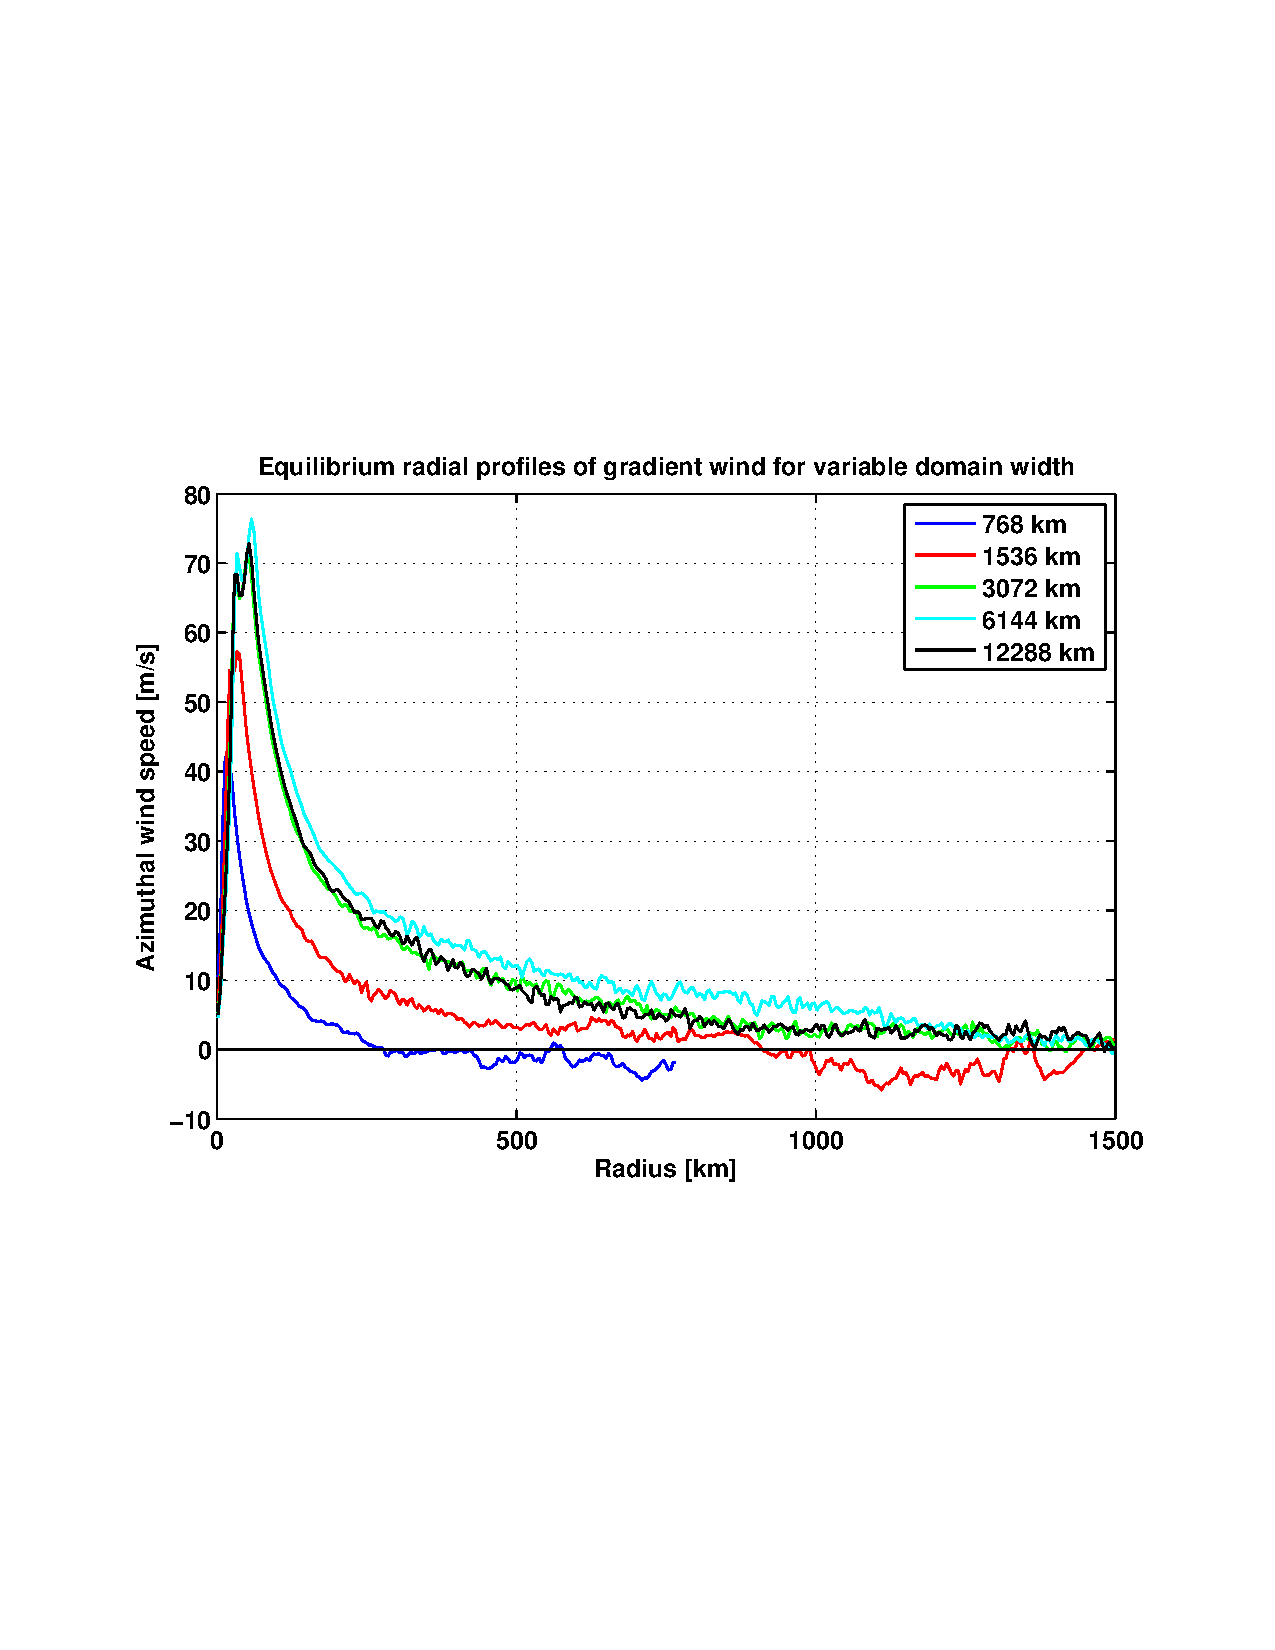
\includegraphics[width=19pc,angle=0]{FIGURES/Domain_size.pdf}
  \noindent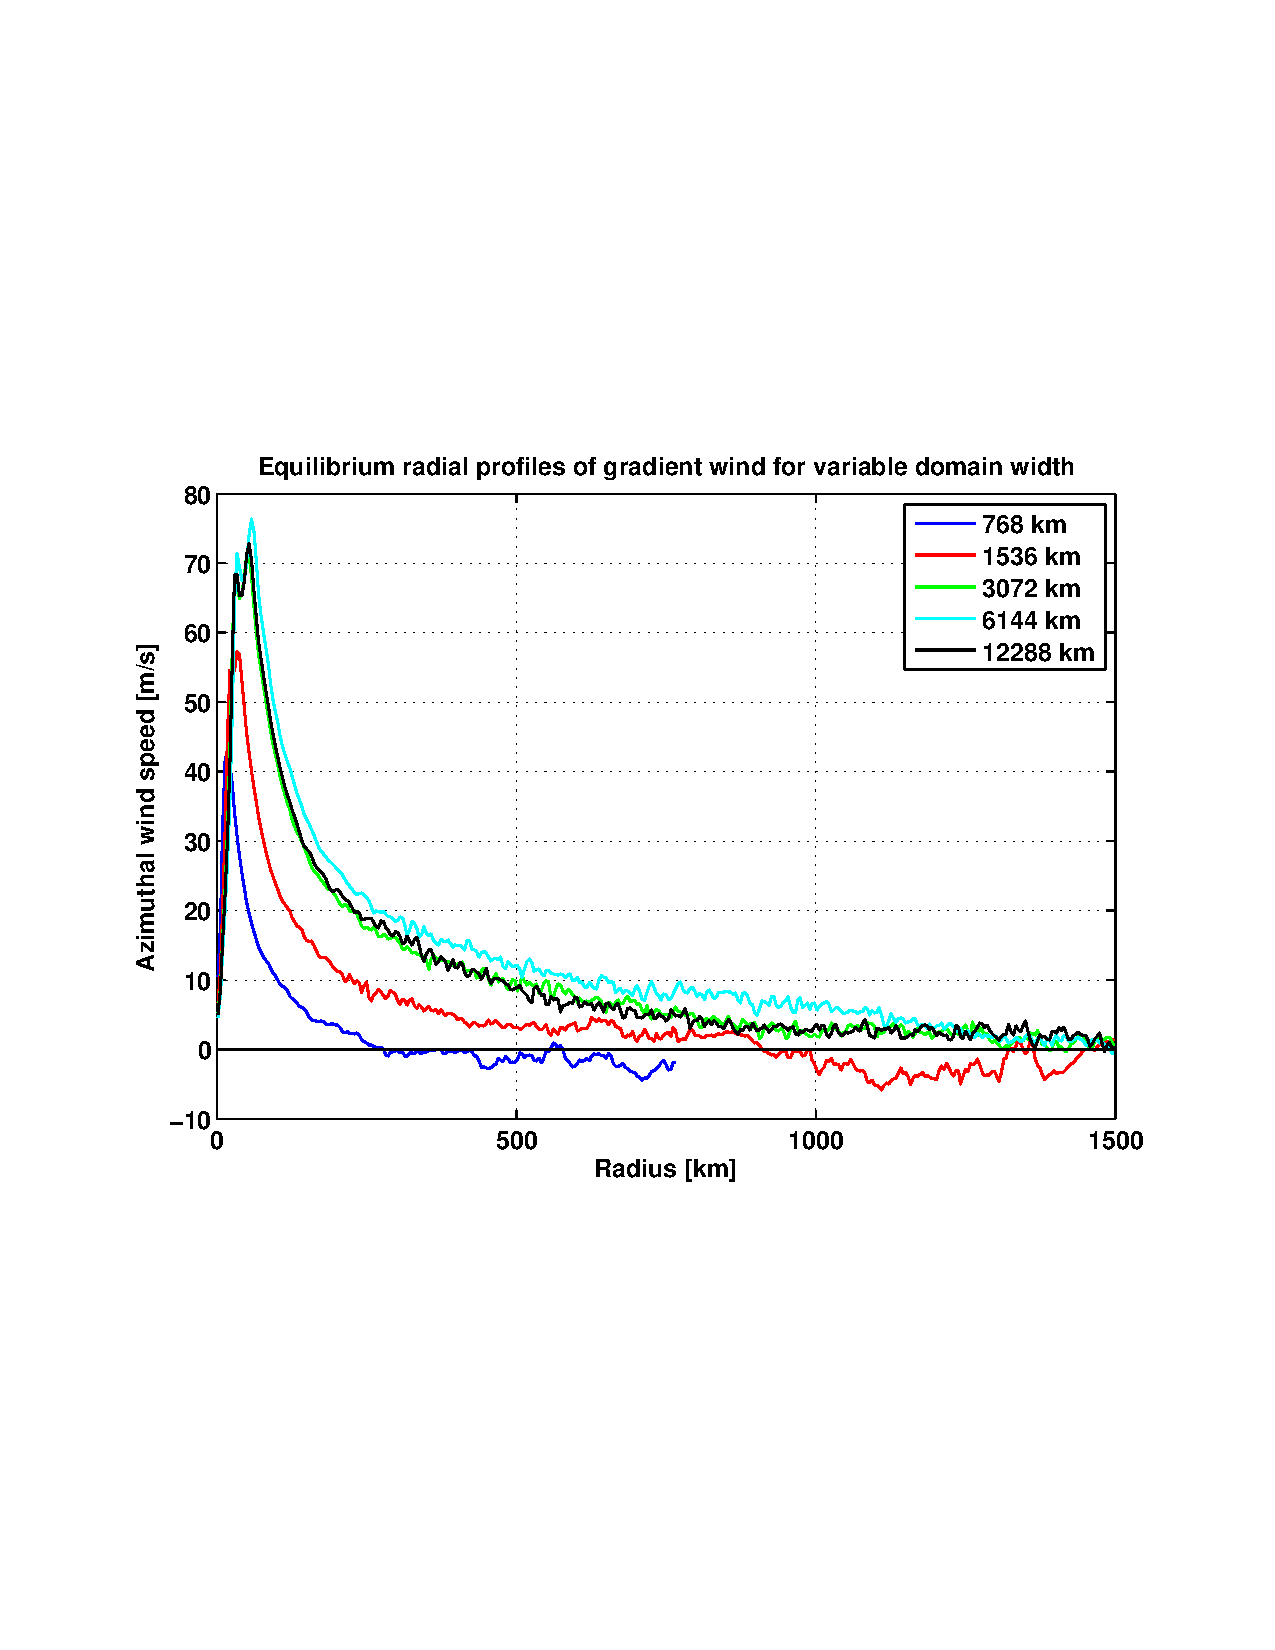
\includegraphics[width=15cm,height=15cm]{FIGURES/Domain_size.pdf}
\caption{Equilibrium radial gradient wind profiles as a function of domain width.  Note the convergence beyond $L_{domain} \approx 3000 \; km$.}
\label{fig:domainsize}
\end{figure}

\begin{figure}[h!]
\centering
%  \noindent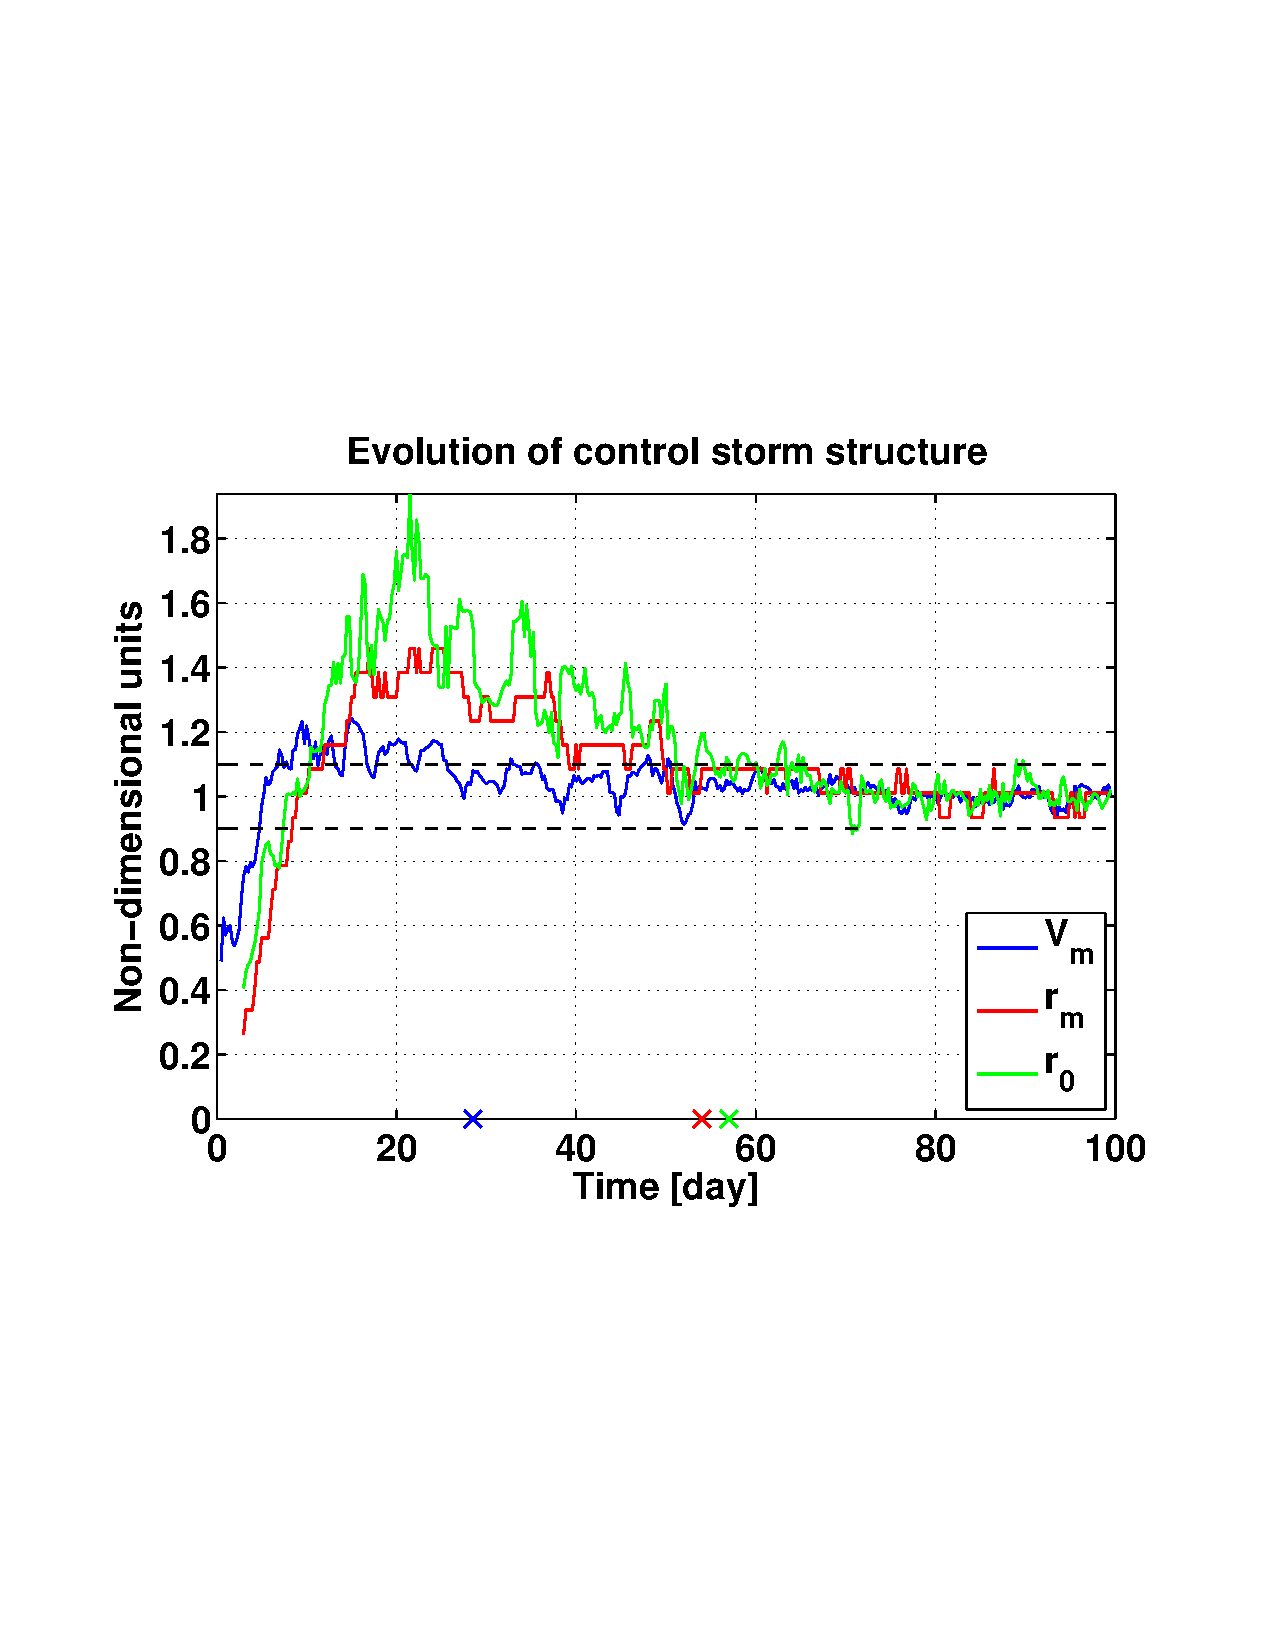
\includegraphics[width=19pc,angle=0]{FIGURES/Control_run.pdf}
  \noindent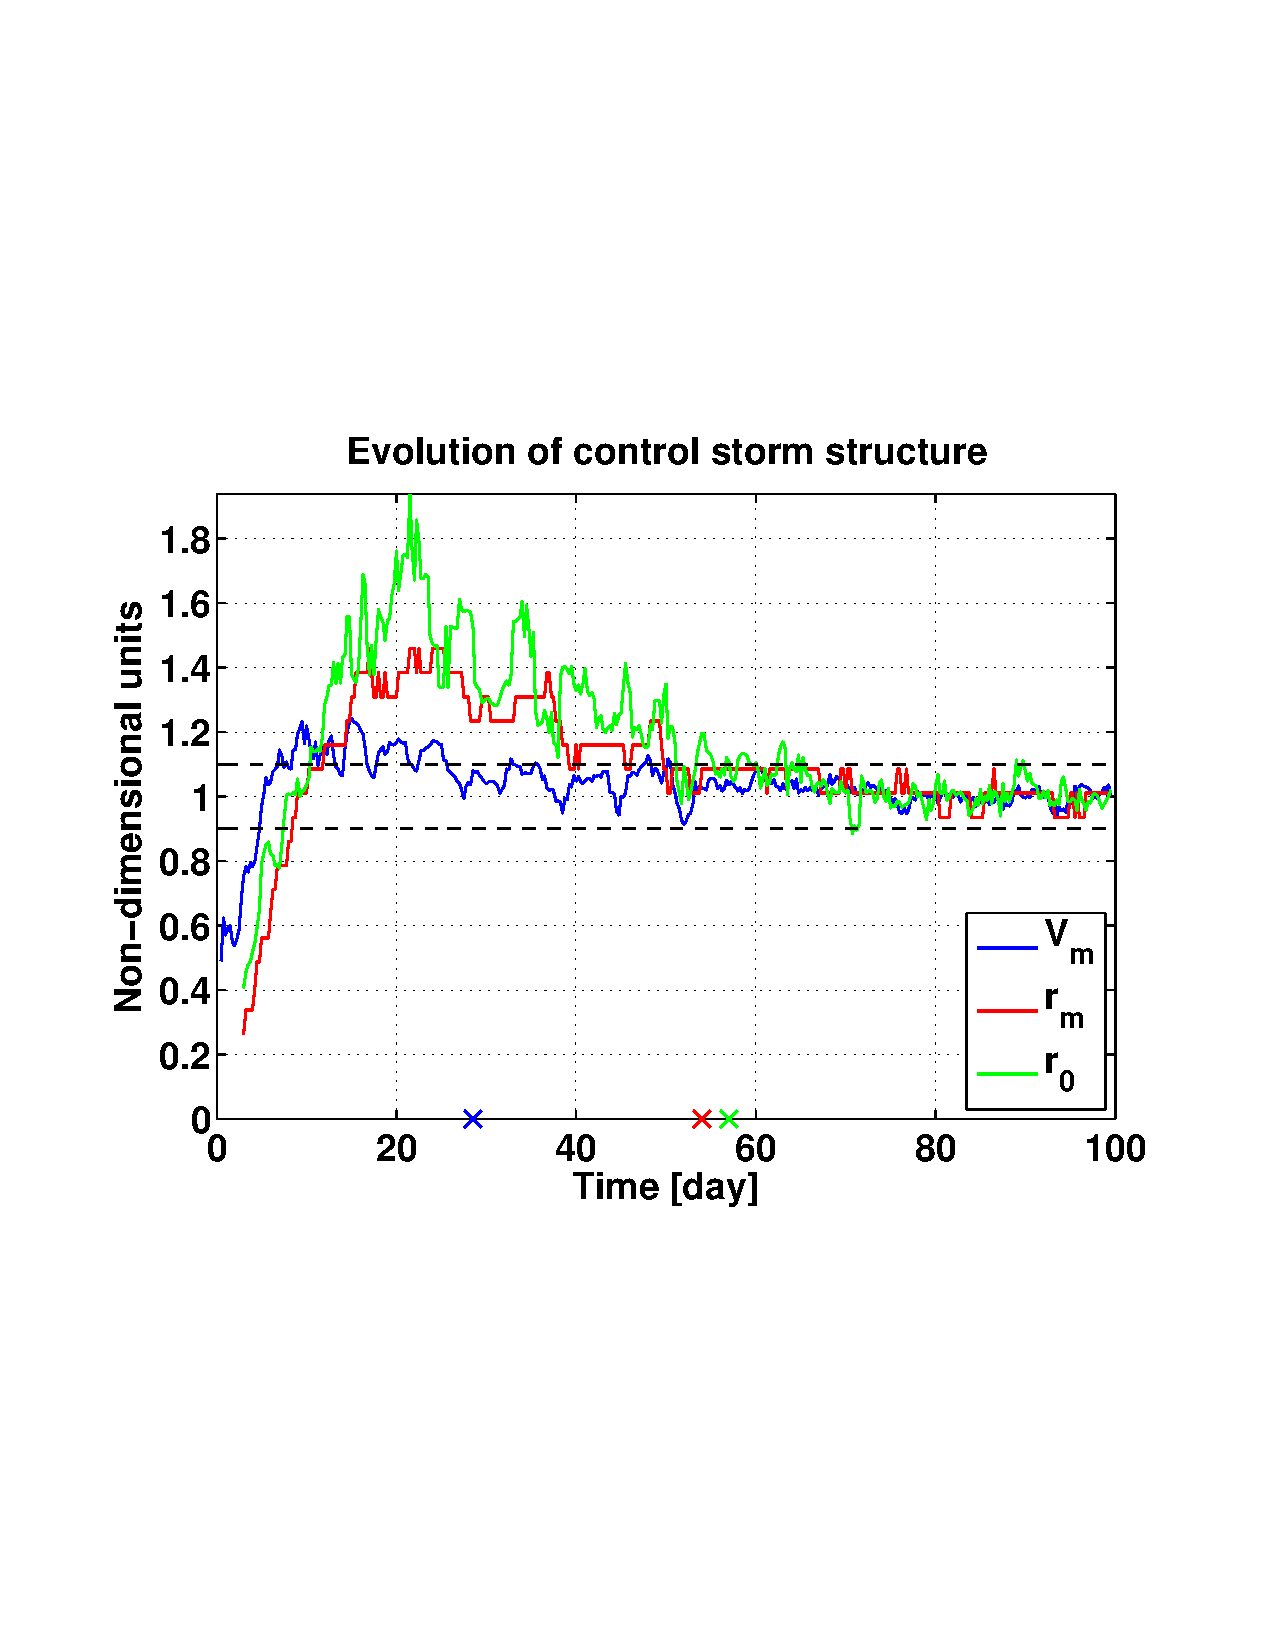
\includegraphics[width=15cm,height=15cm]{FIGURES/Control_run.pdf}
\caption{Control simulation time evolution of 1-day running mean $V_m$, $r_m$, and $r_0$ normalized by their respective equilibrium values (i.e. 70-100 day mean): $V^*_m = 73 \; ms^{-1}, r^*_m = 53 \; km, r^*_0 = 1150 \; km$. Markers along the x-axis denote respective time-scales to equilibration, defined as time where the 30-day running mean is within 10\% of the equilibrium value (black dashed lines). Note: $r_m$ and $r_0$ are not well-defined during genesis and thus are not displayed for $V_m<.7V^*_m$.}
\label{fig:timeseries}
\end{figure}

\begin{figure}[h!]
\centering
%  \noindent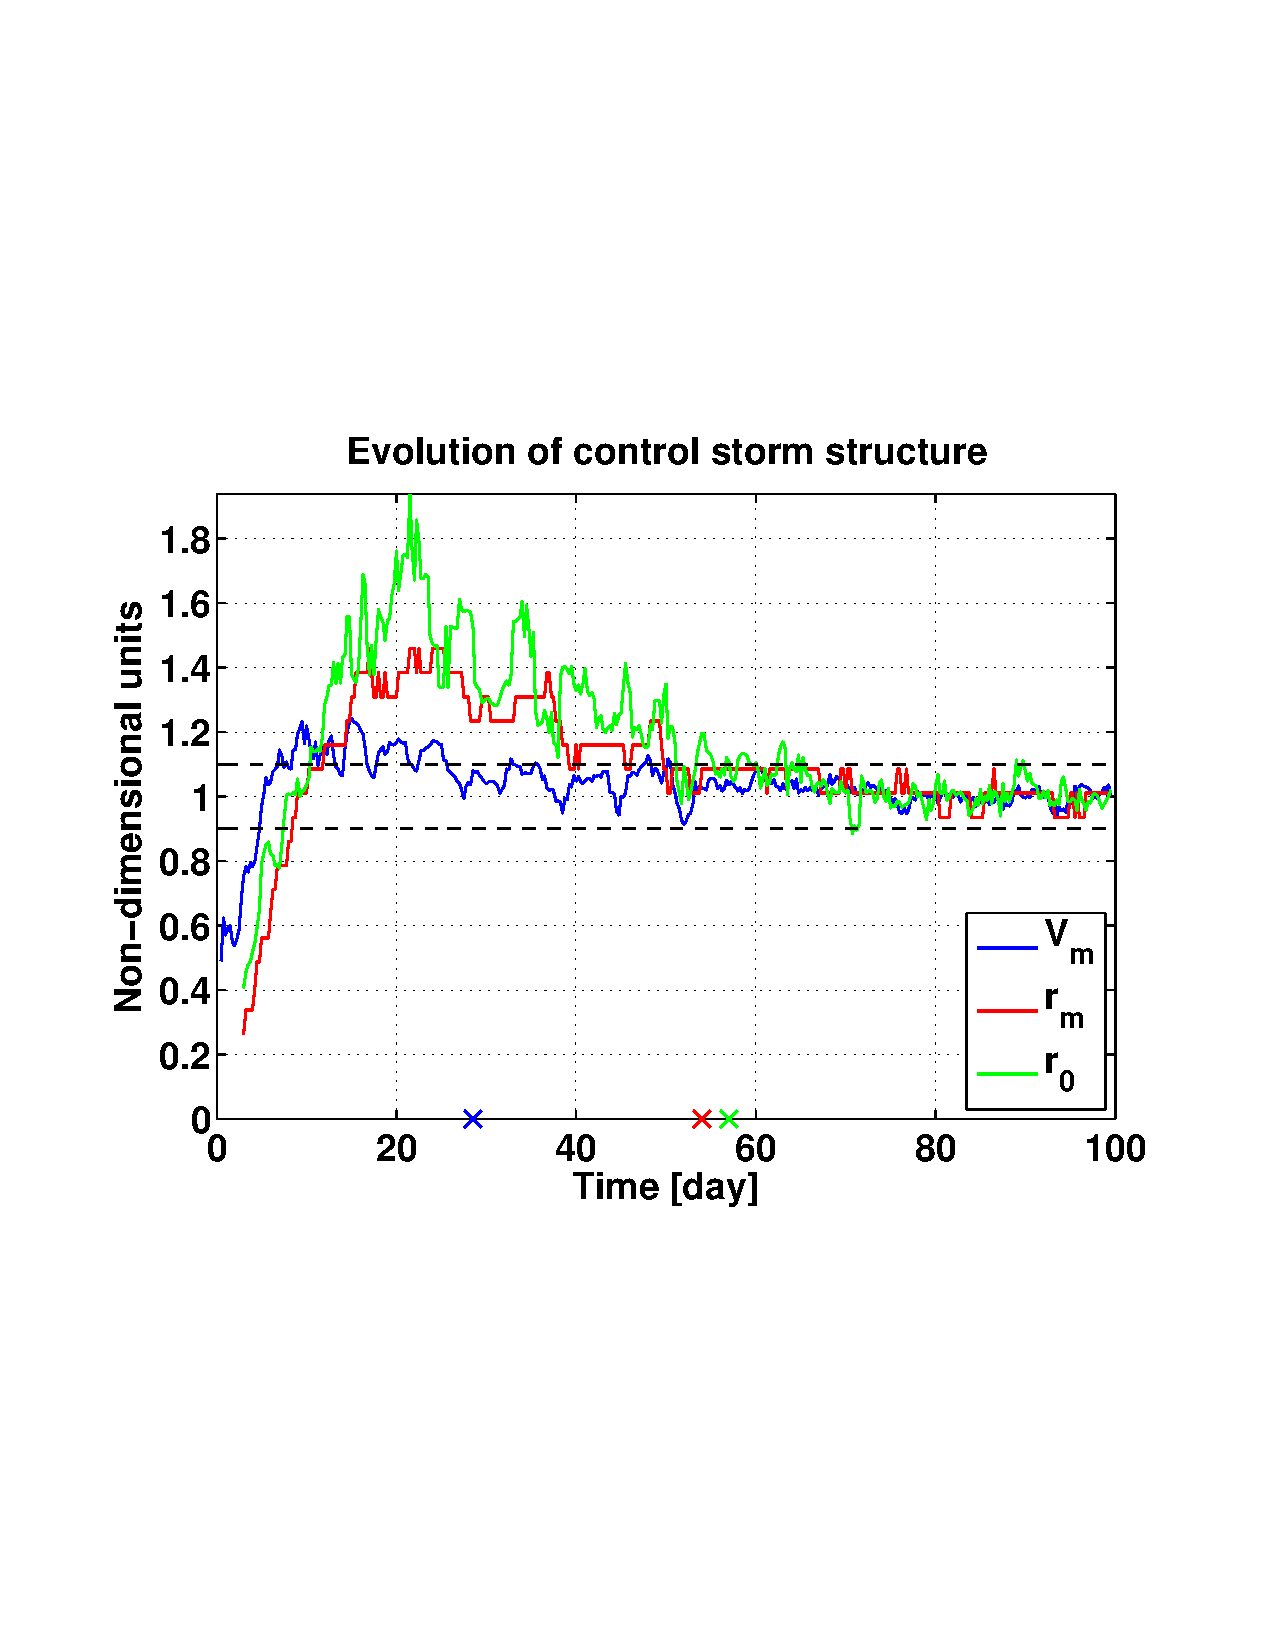
\includegraphics[width=19pc,angle=0]{FIGURES/Control_run.pdf}
  \noindent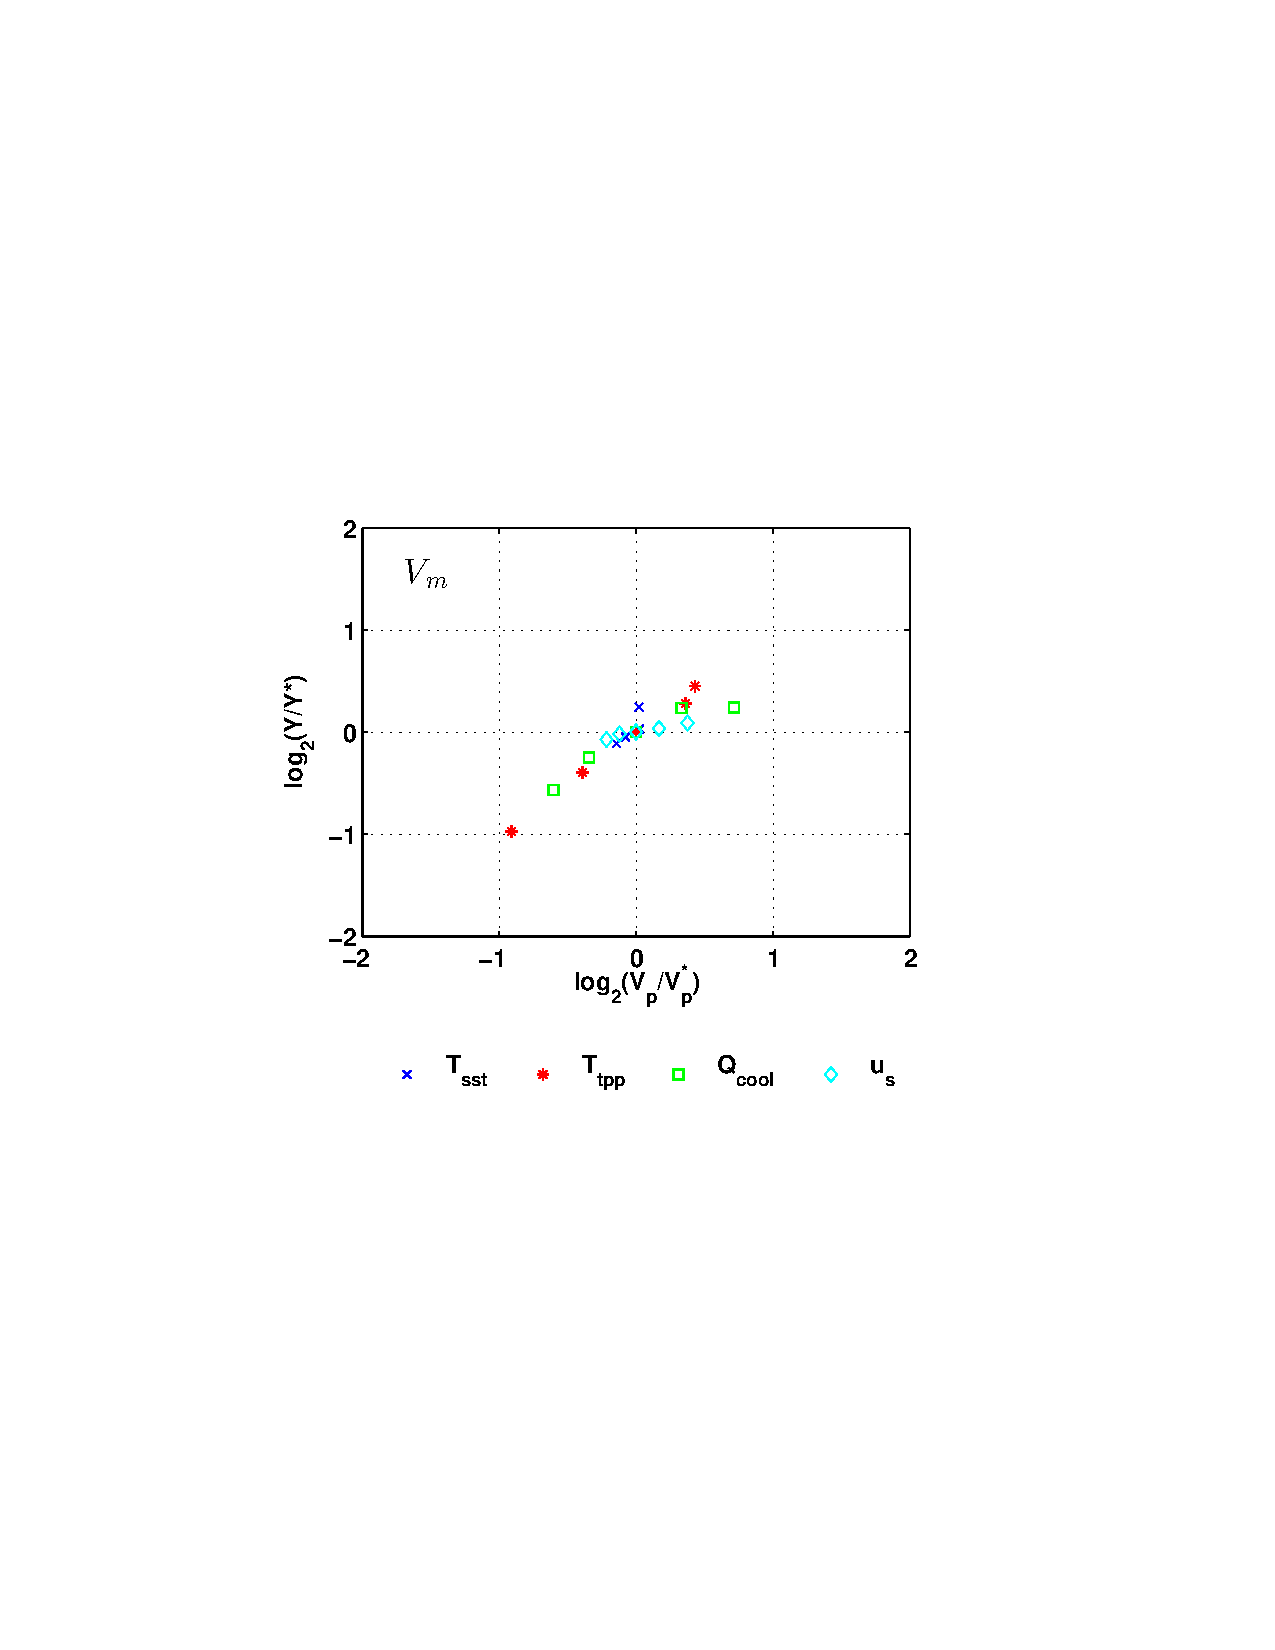
\includegraphics[width=15cm,height=20cm]{FIGURES/MPI_collapse_V.pdf}
\caption{Scaling of the equilibrium value of $V_m$ (ordinate) with the potential intensity (abscissa). Both quantities are normalized by their respective control values denoted by an asterisk ($*$; $V^*_p = 93 \; ms^{-1}$). Colored shape denotes the input parameter varied from among the four parameters on which the potential intensity depends (Eq. \eqref{eq:vpot3}). Scaling is shown in base-2 log-log space, such that a 1-unit increase (decrease) represents doubling (having).  Thus, a straight line with unit slope indicates that a doubling of $V_p$ is associated with a doubling of $Y$.}
\label{fig:mpicollapse_V}
\end{figure}

\begin{figure}[h!]
\centering
%  \noindent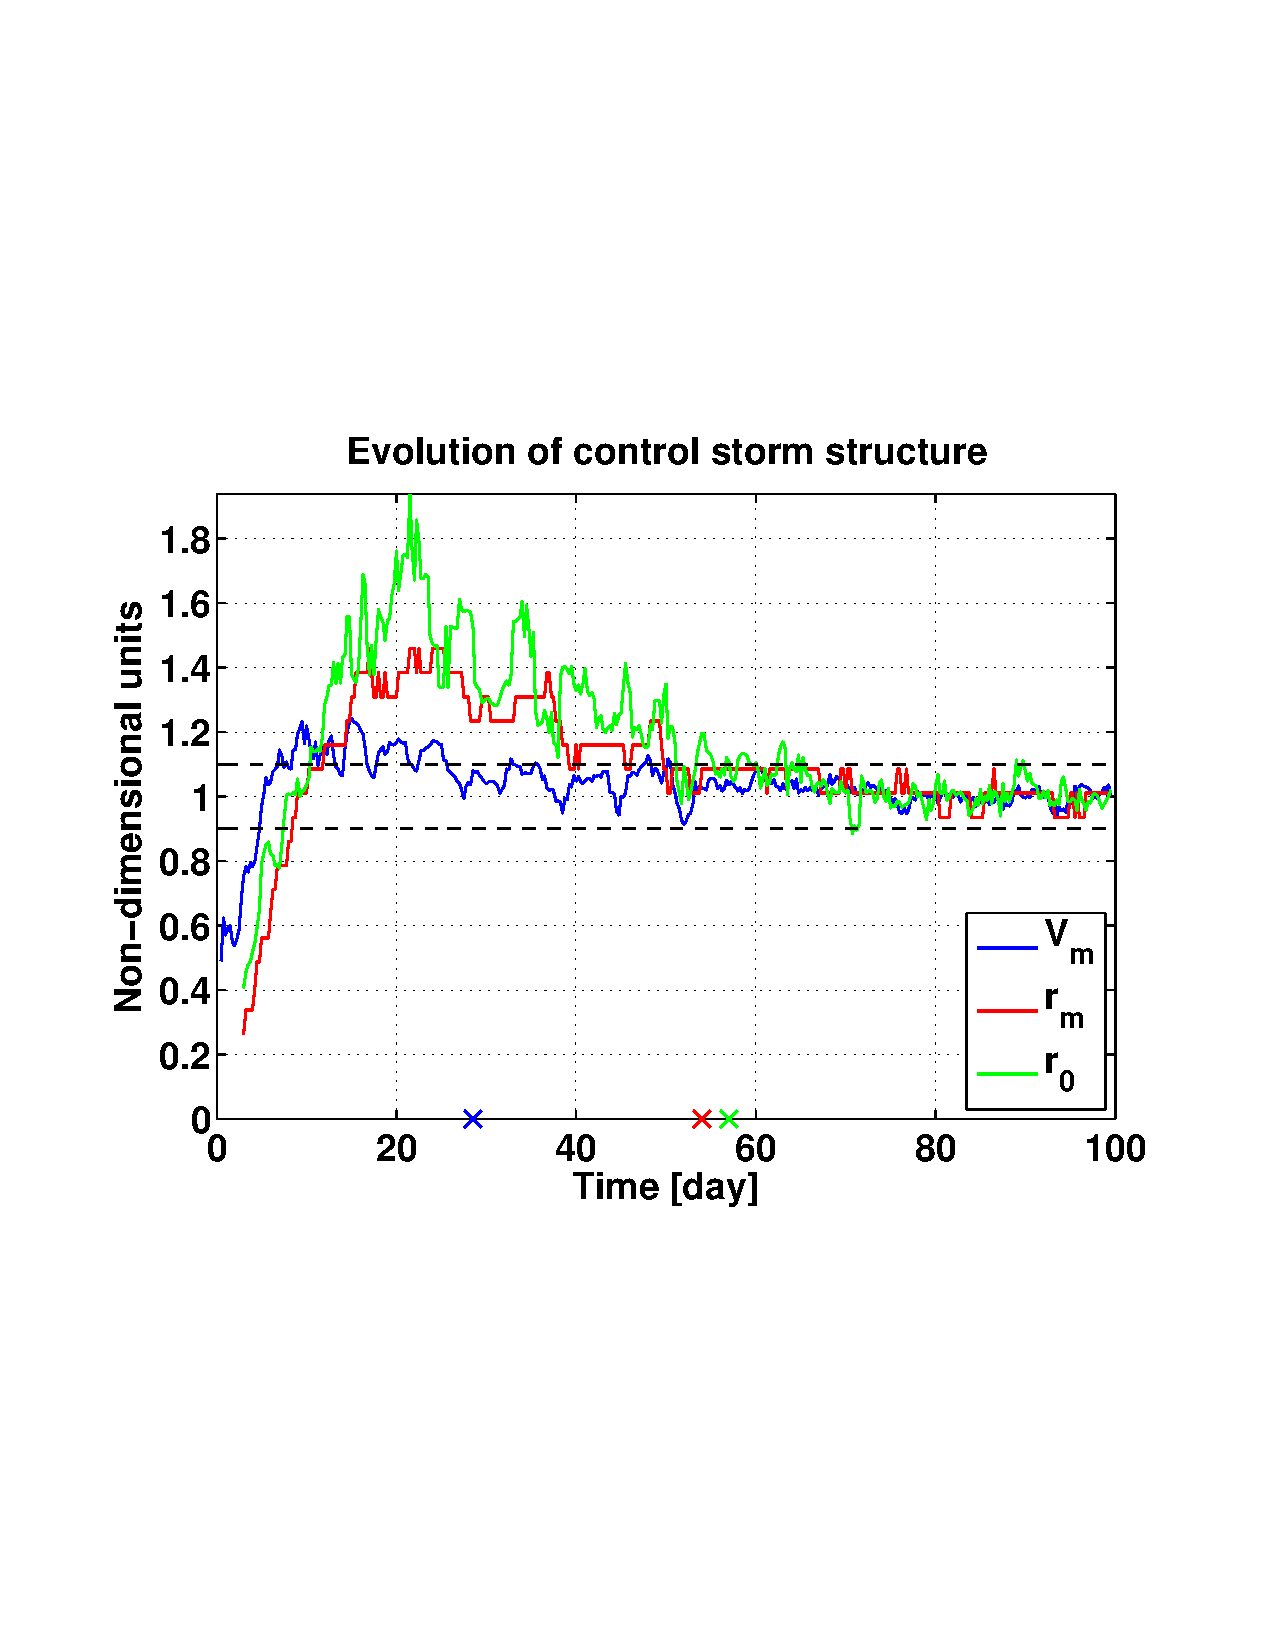
\includegraphics[width=19pc,angle=0]{FIGURES/Control_run.pdf}
  \noindent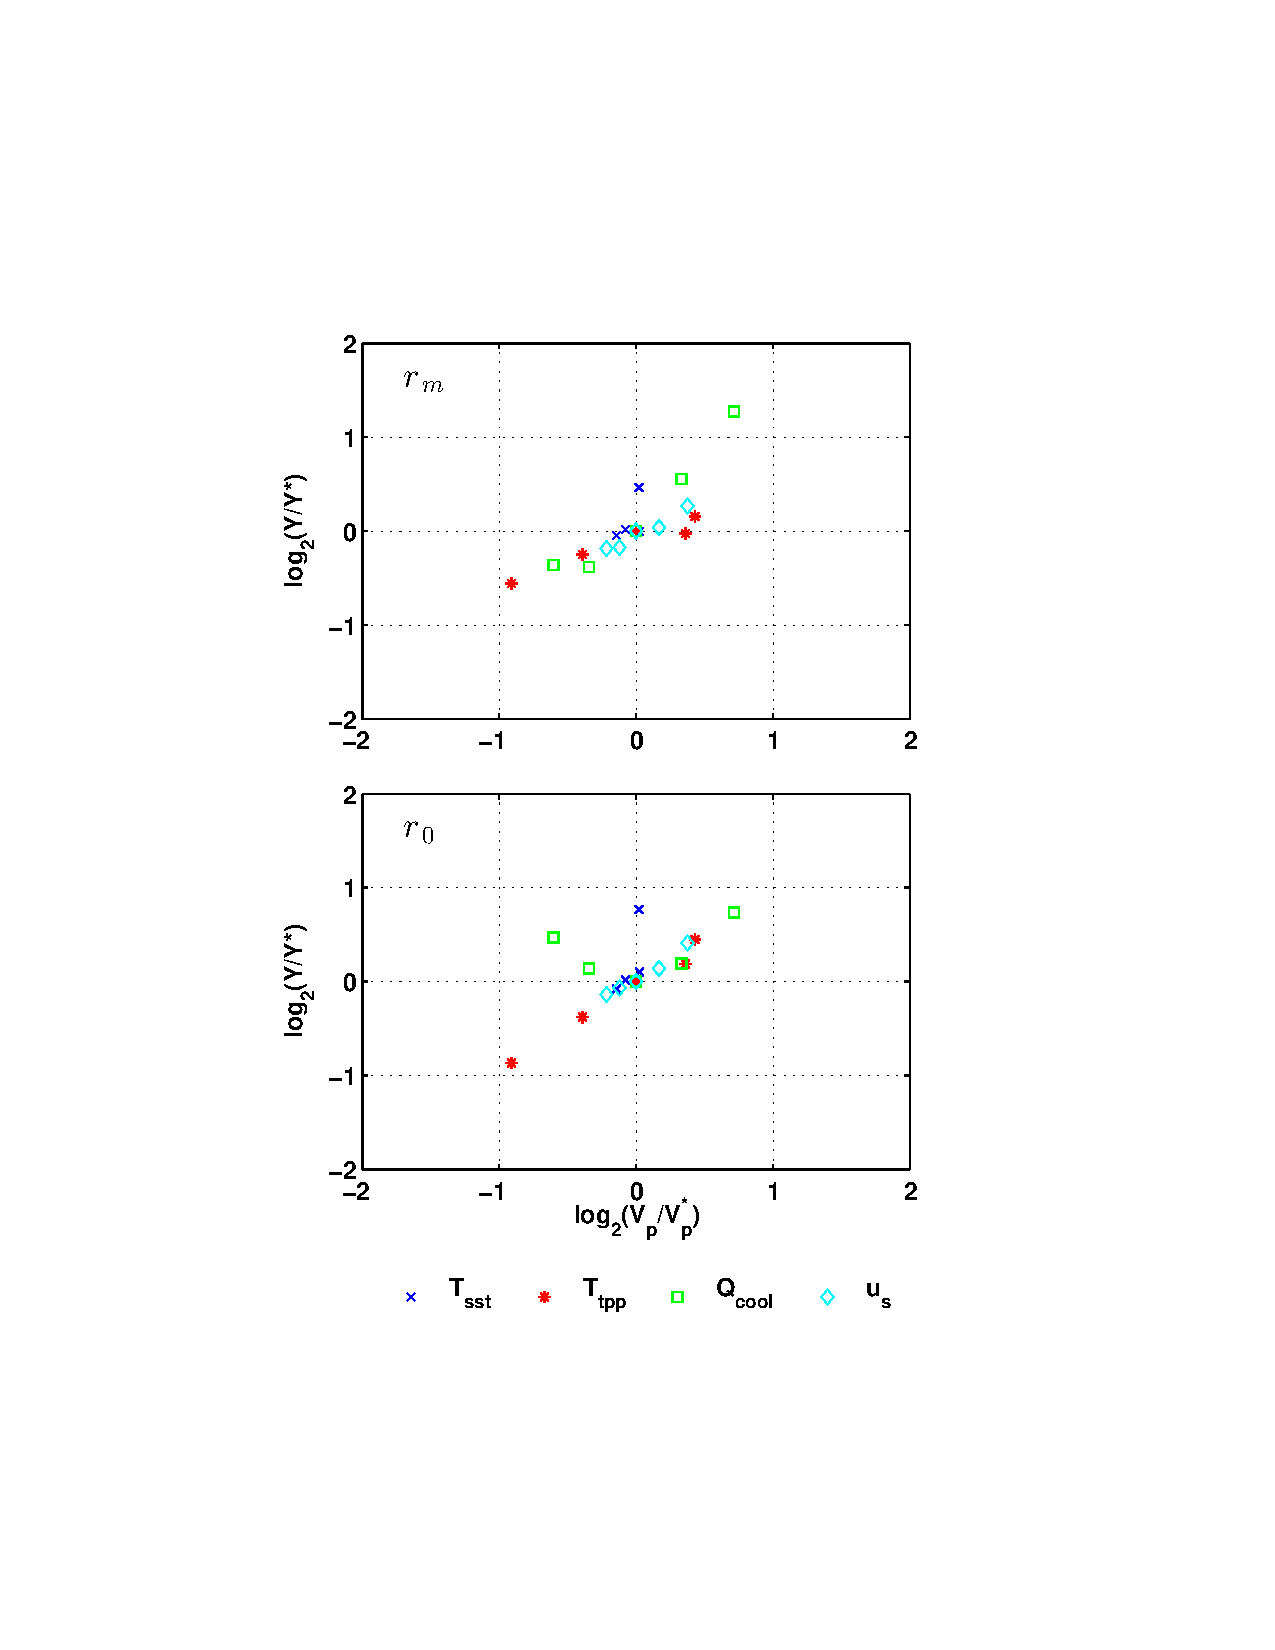
\includegraphics[width=15cm,height=20cm]{FIGURES/MPI_collapse_r.pdf}
\caption{As in Figure \ref{fig:mpicollapse_V}, but for $r_m$ (top) and $r_0$ (bottom).}
\label{fig:mpicollapse_r}
\end{figure}

\begin{figure}[h!]
\centering
%  \noindent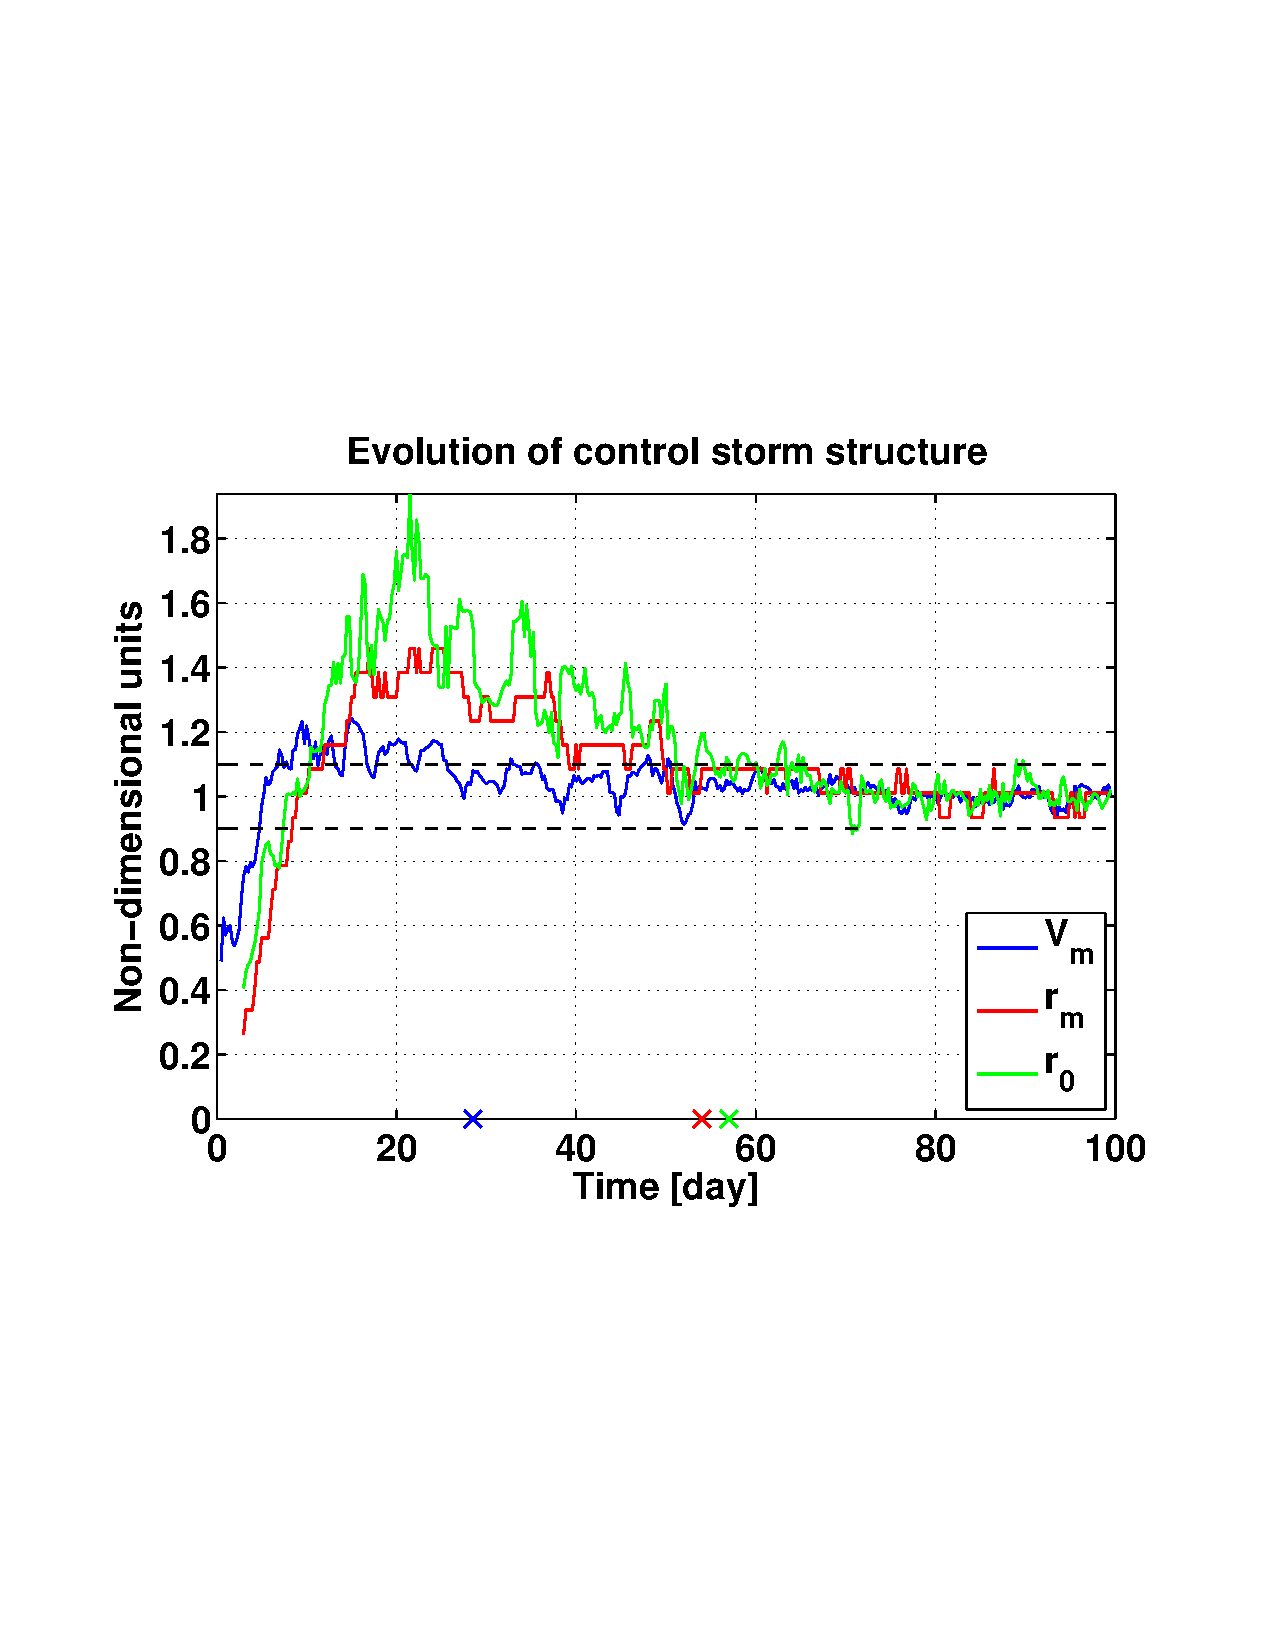
\includegraphics[width=19pc,angle=0]{FIGURES/Control_run.pdf}
  \noindent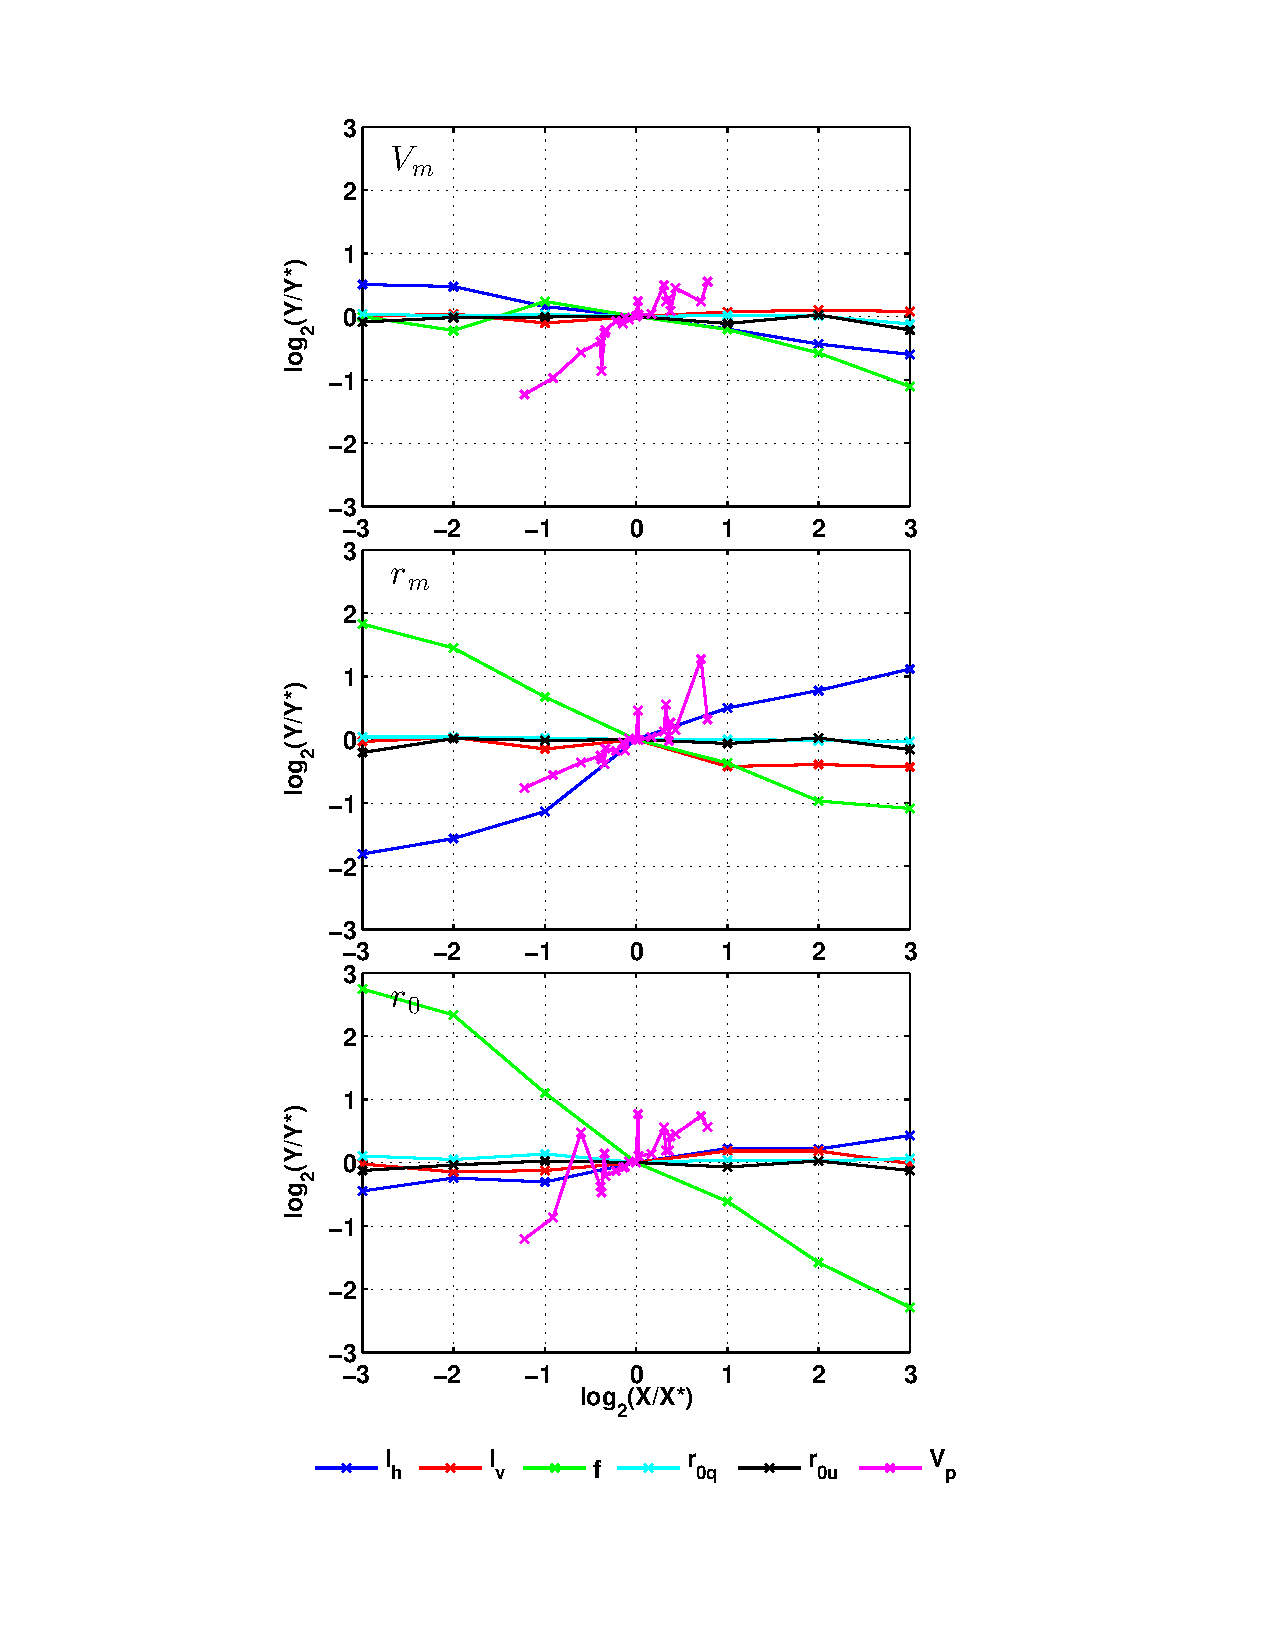
\includegraphics[width=15cm,height=20cm]{FIGURES/Dimensional_scaling.pdf}
\caption{Scaling of the equilibrium value of each structural variable $Y$ (ordinate) with relevant dimensional parameters, $X$ (absicssa). All quantities are normalized by their respective control values denoted by an asterisk ($*$). Plot layout as in Figure \ref{fig:mpicollapse}.}
\label{fig:dimscaling}
\end{figure}

\begin{figure}[h!]
\centering
%  \noindent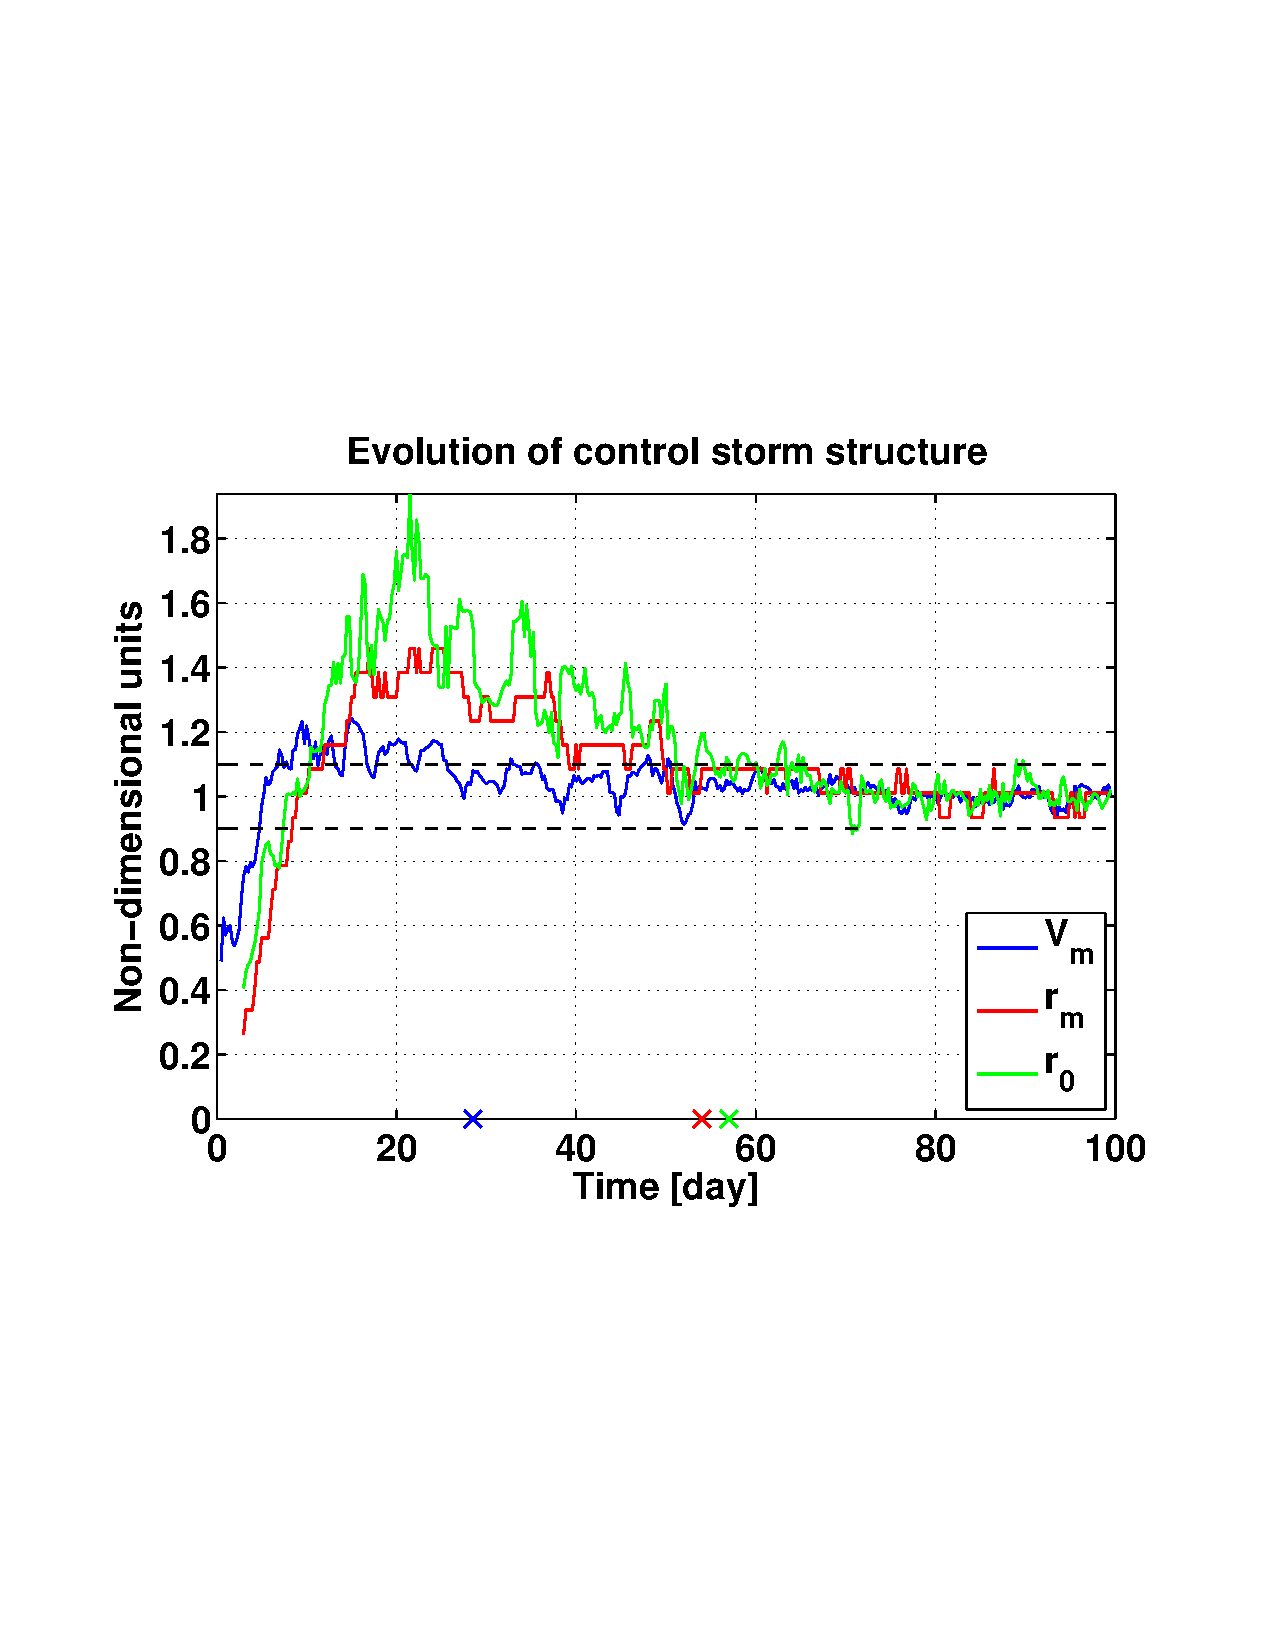
\includegraphics[width=19pc,angle=0]{FIGURES/Control_run.pdf}
  \noindent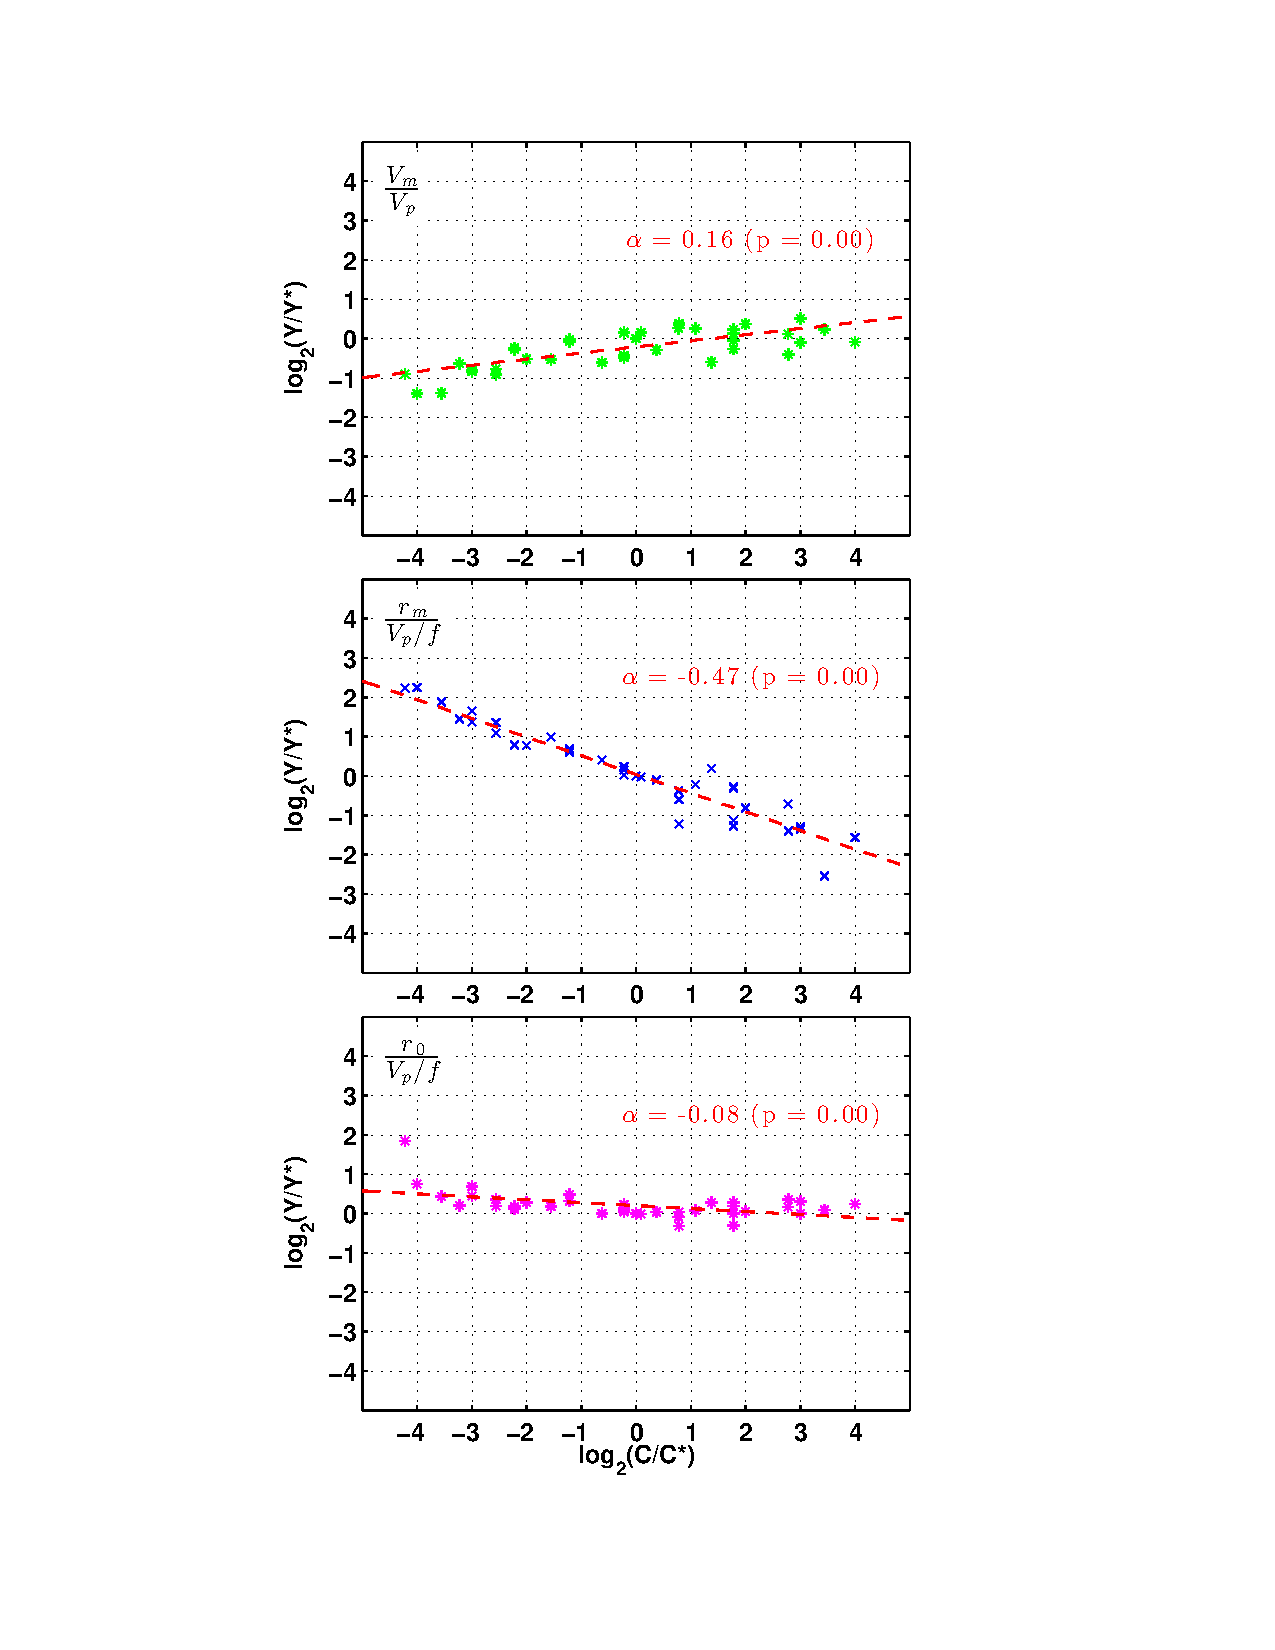
\includegraphics[width=15cm,height=20cm]{FIGURES/Nondimensional_scaling.pdf}
\caption{Scaling of the equilibrium value of each structural variable non-dimensionalized by an appropriate dimensional scale ($V_p$ for $V_m$; $\frac{V_p}{f}$ for $r_m$ and $r_0$), $Y$, with the non-dimensional number $C = \frac{V_p}{fl_h}$ (see text for details). All quantities are normalized by their respective control values denoted by an asterisk ($*$; $C^* = 1240$). Plot layout as in Figure \ref{fig:mpicollapse}.  Linearly-regressed slopes, corresponding to the estimated scaling exponent in \eqref{eq:buckpipowerlaw}, and associated p-values shown in red.}\label{fig:nondimscaling}
\end{figure}

%%SAMPLE
%BEGIN COMMENT
\begin{comment}
\begin{figure}[t]
  \noindent\includegraphics[width=19pc,angle=0]{/Users/drchavas/Documents/LaTeX/AMS_LaTeX/figure01.pdf}\\
  \caption{Enter the caption for your figure here.  Repeat as
  necessary for each of your figures. Create a figures directory and
  place all figures in that directory. Figure from Knutti et al. (2008).}\label{f1}
\end{figure}
%%%%%%%%%%%%%%%%%%%%%%%%%%%%%%%%%%%%%%%%%%%%%%%%%%%%%%%%%%%%%%%%%%%%%
% TABLES
%%%%%%%%%%%%%%%%%%%%%%%%%%%%%%%%%%%%%%%%%%%%%%%%%%%%%%%%%%%%%%%%%%%%%
\begin{table}[t]
\caption{This is a sample table caption and table layout.  Enter as many tables as
  necessary at the end of your manuscript. Table from Lorenz (1963).}\label{t1}
\begin{center}
\begin{tabular}{ccccrrcrc}
\hline\hline
$N$ & $X$ & $Y$ & $Z$\\
\hline
 0000 & 0000 & 0010 & 0000 \\
 0005 & 0004 & 0012 & 0000 \\
 0010 & 0009 & 0020 & 0000 \\
 0015 & 0016 & 0036 & 0002 \\
 0020 & 0030 & 0066 & 0007 \\
 0025 & 0054 & 0115 & 0024 \\
\hline
\end{tabular}
\end{center}
\end{table}
%END COMMENT
\end{comment}

%
\end{document}